\chapter{Memory formation in Alzheimer's Disease}
\section{Introduction}

\section{Material and Methods}

\subsection{Animals and vectors}
All animals were housed in groups of 3--5, with a 12-hour light/dark cycle. Food and water are provided \textit{ad libitum} to all animals. Experiments were performed during the light phase of the circadian cycle. Mice were at least 8 weeks old at the beginning of all experiments. All experiments were conducted in accordance to the Hospital for Sick Children Animal Care and Use Committee.

\subsubsection{TgCRND8 mice}
TgCRND8 mice were developed at the Center of Research for Neurodegenerative Diseases (CRND) and carry a human APP695 transgene with the Swedish (K670N-M671L) and Indiana (V717F) FAD mutations under the regulation of the Syrian hamster prion promoter \citep{chishti01}. Transgenic mice were maintained in a 129S6/SvEvTac background. TgCRND8 was then crossed with either \gls{wt} C57BL/6NTac or GP5.17. \Gls{tg} and \gls{wt} litter-mates of F1 generation were used in the experiments.


\subsubsection{GP5.17 mice}
GP5.17 mice transgenically express the fluorescence calcium indicator GCaMP6f under the Thy1 promoter \citep{dana14}. Offspring of TgCRND8 $\times$ GP5.17 positive of GCaMP6f and negative for \gls{app} were included in the \gls{wt} group. Double positive offspring were included in the \gls{tg} group.


\subsubsection{Viral vectors}
In the TgCRND8 mice, GCaMP6f expression is delivered through \gls{aav}. GCaMP6f expression is controlled by \gls{hsyn} promoter. AAV--DJ--syn--GCaMP6f virus was purchased from Stanford University Gene and Viral Vector Core and used undiluted. 

\subsubsection{\tglu peptide}
To deliver \glu construct (\texttt{YKEGYNVYG}) to target, we attached it to the protein transduction domain of the \gls{hiv} \textit{tat} gene (TAT peptide). The TAT peptide is able to transport across cell membrane and \gls{bbb} through a mechanism which is still unknown \todo{cite TAT}. The \tglu was synthesized from the sequence \texttt{YGRKKRRQRRRYKEGYNVYG}. It was injected in saline solution.


\subsection{Viral Infusion}

Each animal received \gls{ip} injection of atropine (\SI{0.1}{\mg\per\kg}) and chlorohydrate (\SI{400}{\mg\per\kg}) before being secured on a stereotaxic frame. An incision was made on the scalp and the skin was pulled to the side to reveal the skull. Holes were drilled above \gls{la} on the skull for micropipette injection. Virus was loaded into a glass micropipette and gradually lowered to target coordinate. \SI{1.5}{\ul} of virus were injected on each side at a rate of \SI{0.12}{\ul\per\min}, aiming at \gls{la} (\gls{a/p} \SI{-1.4}{\mm}, \gls{m/l} $\pm$\SI{3.5}{\mm}, \gls{d/v} \SI{5.0}{\mm} from Bregma). The micropipette was left in the brain for an extra \SI{10}{\min} before slowly retracted. The incision was sutured and treated with antibiotics. Each animal then received subcutaneous injection of analgesic (ketoprofen, \SI{5}{\mg\per\kg}) before returned to a partially heated clean cage for recovery.

\subsection{Histology}
Placement of lens implants and extent of viral infections was determined by gCaMP6f fluorescence expression \textit{post-mortem}. After all experiments, animals were transcardially perfused with first \gls{pbs} then 4\% \gls{pfa}. The brains were dissected,  kept in 4\% \gls{pfa} overnight, and washed with \gls{pbs}. The brains were then sliced coronally on a vibrotome (\todo{vibrotome info}) to \SI{50}{\um} thickness. Slices containing \gls{la} were then mounted on gelatin-coated glass slides with a hardening mounting media (Permaflour\todo{permaflour info}). The mounted brain slices were assessed under an epi-fluorescence microscope(Nikon\todo{Nikon info}) for histology.


\subsection{Contextual fear conditioning}
Fear conditioning chambers (\SI{31 x 24 x 21}{\cm}; MED Associates, St. Albans, VT) consisted of 2 stainless steel and 2 clear acrylic walls with a stainless steel shock-grid floor (bars \SI{3.2}{\mm} diameter, spaced \SI{7.9}{\mm} apart). A plastic drop-pan containing a 70\% ethanol solution was placed below the grid floor. A fan provided low-level white noise during training and testing in the context. Behaviour was monitored by overhead cameras, which recorded video images of the chambers at \SI{15}{\Hz}. 

Animals underwent contextual fear conditioning three weeks after mini-microscope baseplate implantation. One hour before training, animals received either \tglu peptide (\gls{ip}, \SI{15}{\mmol\per\kg}) or saline injection. A mini-microscope is attached to the animal to record calcium activities during both training and testing of contextual fear conditioning. During training, animals were confined in the chamber for \SI{5}{\minute}. A foot-shock of \SI{0.5}{\mA} was delivered at \SI{4}{\minute} time point. During testing session \SI{24}{\hour} later, animals were placed back in the training environment for \SI{10}{\minute}. 

\subsection{Animal tracing}
\todo{Animal tracing method}
Videos of animal behaviours were encoded as grey-scale images. Due to a dark background, overlaying mini-microscope wire and commutators and changing shadows, no simple feature is able to reliably identify the animal from the background. Instead, we used multiple features, calculate the distribution of the features in tracked animals, and use all the features together to estimate the position of the animal for each frame. During model fitting, distribution of every feature was estimated with a Gaussian kernel, with a bandwidth calculated using Silverman's rule of thumb\todo{cite Silverman 1986} as: $1.06\sigma n^{-\frac{1}{5}}$, where $\sigma$ is the standard deviation of the samples, and $n$ is the number of samples.

\subsubsection{Features}

\paragraph{Pixel intensity.} Pixel intensity at animal's position. This feature tries to capture the animal's fur colour.

\paragraph{Normed pixel intensity.} Normalized pixel intensity of animal's position, where the frame is normalized to zero mean and unit standard deviation. This feature tries to capture animal's fur colour when the illumination in the chamber varies across frames.

\paragraph{Foreground pixel intensity.} Pixel intensity difference between foreground and background images at the animal's position. The background image of the environment was generated by taking the mean pixel density across time. This feature tries to separate animals from any background pixels with similar colour.

\paragraph{Difference to low pass intensity.} Pixel intensity difference between foreground image and low-pass filtered foreground image (\SI{10}{\mm} window) at animals position. This feature tries to capture the fact that the animal's colour is close to uniform, therefore eliminates sporadic noise pixels with similar colour.

\paragraph{Speed.} Distance between animal's positions in two consecutive frames. 

\paragraph{Change in intensity.} Difference of pixel intensity at animal's positions in two consecutive frames. This feature captures the fact that animal's colour is relative consistent between frames.

\paragraph{Change in intensity (blurred).} Similar to change in intensity, but using Gaussian blurred images (\SI{10}{\mm} window) to remove effect of random noise.

\paragraph{Magnitude of acceleration.} Magnitude of acceleration vector, which is calculated as the vector difference of two consecutive velocity calculations. 

\paragraph{Segmentation area.} Edges in the frame is detected (Canny, lower threshold=100, higher threshold=200). The resulting image is then morphologically closed (6 iterations) to remove sporadic edges. The area enclosing the position of the animal is then calculated. This feature tries to capture the size of the animal.

\subsubsection{Tracking}

The animal's position over time is modeled as a \gls{hmm}, as show in Figure \ref{f.ad.hmm} where animal's true position at time $i$ is represented by the hidden variables $z_i$, and we can make measurements using the various features above and get measurements at each time point, represented as $x_i$. 

\begin{figure}[h]
    
\begin{tikzpicture}[biglatent/.style={latent, minimum width={width("$z_{n+1}$")+6pt}}, bigobs/.style={biglatent, fill=gray!25}]
    \node[biglatent] (z0) {$z_0$};
    \node[biglatent, right=of z0] (z1) {$z_{1}$};
    \node[biglatent, right=of z1] (z2) {$z_2$};
    \node[right=of z2] (z25) {\Large{$\cdots$}};
    \node[biglatent, right=of z25] (z3) {$z_{n-1}$};
    \node[biglatent, right=of z3] (z4) {$z_{n}$};
    \node[biglatent, right=of z4] (z5) {$z_{n+1}$};
    \node[right=of z5] (z55) {};

    \foreach \t [count=\i from 0] in {0,1,2,n-1,n,n+1}{
        \node[bigobs, below=of z\i] (x\i) {$x_{\t}$};
        \edge {z\i} {x\i};
    };
    \node[right=of x2] (x25) {\Large{$\cdots$}};
    \edge {z0} {z1};
    \edge {z1} {z2};
    \edge {z2} {z25};
    \edge {z25} {z3};
    \edge {z3} {z4};
    \edge {z4} {z5};
    \edge {z5} {z55};

\end{tikzpicture}

    \caption{\gls{hmm} model for tracking animal. Animal's true position at time $i$ is represented by the latent variables $z_i$, measurements of the animal's position is represented by $x_i$. \label{f.ad.hmm}}
\end{figure}

Using particle filter, we approximate the posterior distribution $f_{z_n}(z_n|X_n)$ with $L$ particles at $\{a^i\}_{i=1}^L$ with weights $\{w^i\}_{i=1}^L$, such that the posterior distribution can be approximated with a mixture of Dirac delta function: 
\begin{equation} \label{zn_approx}
    f_{z_n}(z_n|X_n) \approx \sum_{i=1}^Lw_n^i\delta(z_n - a_n^i)
\end{equation}

On the other hand, using Bayes rule and independencies form the \gls{hmm} structure, we have:
\begin{align*}
    f_{z_n}(z_n|X_n) &\propto f_{x_n}(x_n|z_n, X_{n-1}) \cdot f_{z_n}(z_n|X_{n-1}) \\
                     &= f_{x_n}(x_n|z_n) \int f_{z_n}(z_n|z_{n-1})f_{z_{n-1}}(z_{n-1}|X_{n-1})dz_{n-1}  \\
                     &\approx f_{x_n}(x_n|z_n) \int f_{z_n}(z_n|z_{n-1})\cdot \sum_{i=1}^Lw_{n-1}^i\delta(z_{n-1}-a_{n-1}^i)dz_{n-1} \\
                     &= f_{x_n}(x_n|z_n)  \sum_{i=1}^Lw_{n-1}^i \int f_{z_n}(z_n|z_{n-1})\delta(z_{n-1} - a_{n-1}^i)dz_{n-1} \\
                     &= f_{x_n}(x_n|z_n) \sum_{i=1}^Lw_{n-1}^if_{z_n}(z_n|a_{n-1}^i) 
\end{align*}
where the probability distribution $f_{x_n}(x_n|z_n)$ is the measurement model, which we approximate with the normalized product of all feature distributions. The motion model $f_{z_n}(z_n|z_{n-1})$ is approximated with the distribution of speed at all directions. Conbined with (\ref{zn_approx}), we can find $\{a_n^i\}_{i=1}^L$ by sampling from the mixture $\sum_{i=1}^Lw_{n-1}^if_{z_n}(z_n|a_{n-1}^i)$, and calculate $w_n^i = f_{x_n}(x_n|a_n^i)$. The center of mass of all particles is used as an estimate of the animal's position $z_n$. This process is then iterated for all frames to track the mouse's position in one behavioural video.

\subsection{Analysis}

\subsubsection{Freezing behaviour}
Freezing behaviour of the mice during first 5 minutes of contextual fear memory testing were assessed by an experimenter who is blind to the genotype and treatment of the mice. Frame-to-frame timestamps for the beginning and end of freezing periods were recorded.

\subsubsection{Cell activity}

All traces were normalized to have zero median and unit noise standard deviation. The noise standard deviation was estimated from median absolute deviation of the trace. The \gls{snr} were calculated as the ratio of maximum signal intensity and noise standard deviation. Only traces with more than 10 \gls{snr} and animals with more than 20 cells are included in the analysis. The average activity of a cell was calculated by the area under the calcium trace above 3 standard deviation of the noise divided by duration.

\subsubsection{Mutual information}

The mutual information measurement of two random variables represents the degree of relatedness between them. The mutual information between the calcium trace for each cell $C$, a continuous random variable and the freezing state of the animal $F$, a discrete random variable, is defined as:
\begin{equation*}
    I(C, F) = \int\limits_{c \in C} \sum_{f \in F} P(c,f)\log\frac{P(c,f)}{P(c)P(f)}dc
\end{equation*}
To estimate the mutual information between freezing and cell activity, we used the \gls{kl} twice to estimate the entropy of calcium trace $H(C)$ and the conditional entropy $H(C|F)$ \citep{ross14, victor02}, and calculated the mutual information using the identity:
\begin{equation} \label{cond_h}
    I(C, F) = H(C) - H(C|F)
\end{equation}
The \gls{kl} is a nearest-neighbour entropy estimator. Given a data point $C_{i,0}$ from a continuous random variable and its m\textsuperscript{th} nearest neighbour $C_{i,m}$, we define $V_{i,m}$ as the volume of ball centered at $C_{i,0}$ with a radius equal to the distance between $C_{i,0}$ and $C_{i,m}$. The entropy of $C$ can be estimated as:
\begin{equation} \label{est_h}
    H(C) \approx \langle \log V_{i,m}^F\rangle + \varphi(N) - \varphi(m)
\end{equation}
where $N$ is the number of samples, and $\langle\cdot\rangle$ denotes the average over $1\ldots N$, and $\varphi$ is the digamma function \todo{reference digamma}. Similarly, we can calculate the entropy for the conditional entropy $H(C|F)$:
\begin{equation} \label{est_cond_h}
    H(C|F) \approx \langle \log V_{i,k}^{F_i} \rangle + \langle \varphi(N_{F_i}) \rangle - \varphi(k)
\end{equation}
where $N_{F_i}$ is the number of samples in the freezing state of $i$\textsuperscript{th} sample, and here we use the $k$\textsuperscript{th} nearest neighbour conditioned on $F_i$ for the calculation.

To avoid sampling error, we fix $k$ for each sample, but change $m$ to the total number of samples between the sample $C_{i,0}$ and its $k$\textsuperscript{th} nearest neighbour conditioned on $F_i$, $C_{i,k}^{F_i}$. Therefore we have:
\begin{equation*}
\log V_{i, m_i} = \log V_{i, k}^{F_i}, \forall i 
\end{equation*}
Plug (\ref{est_h}) and (\ref{est_cond_h}) to (\ref{cond_h}), we have:
\begin{equation*}
    I(C, F) \approx \varphi(N) - \langle\varphi(m_i)\rangle - \langle\varphi(N_{F_i})\rangle + \varphi(k)
\end{equation*}




\subsubsection{Machine learning}

Time-course data for the calcium traces and animal behavioural states are paired and shuffled across time. Activity for each cell is regarded as a single feature. The classifiers are then train and validated using 5-fold cross validation. Specifically, the shuffled data are divided into 5 equal blocks. Each block is held out one at a time, and the classifier is trained using the rest 4 blocks. The hold out block is then used to test the performance of the classifier. The classifier prediction from each block is then concatenated and sorted into the original order. In the analysis, we used two classifiers, a \gls{nbc} and a \gls{gsvm}. 

\paragraph{Poisson Naive Bayes Classifier.}
In a \gls{nbc}, the classifier tries to infer the likelihood of the $i$th target class $T_i$ given the features $\mathbf{x} = (x_1, x_2, \dots, x_n)$. Therefore, we have:
\begin{equation*}
    P(T_i|\mathbf{x}) = \frac{P(T_i, \mathbf{x})}{P(\mathbf{x})}
\end{equation*}
The denominator is not relavent for classification purposes, since it does not depend on the target class $T_i$. Therefore, repeatedly applying the chain rule, we have:
\begin{align*}
    P(T_i|x_1, \dots, x_n) &\propto P(x_1, \dots, x_n, T_i) \\
                           &= P(x_1|x_2 \dots, x_n, T_i) P(x_2, \dots, x_n, T_i) \\
                           &\vdots \\
                           &= P(x_1|x_2, \dots, x_n, T_i)  P(x_2|x_3, \dots, x_n, T_i) \ldots  P(x_{n-1}|x_n, T_i)  P(x_n|T_i)  P(T_i) \\
                           &= P(T_i)  \prod_{k=1}^{n-1} P(x_k|x_{k+1}, \dots, x_n, T_i)
\end{align*}
To make the product trackable, \gls{nbc} discards the interaction between all the features, and assumes the features are conditionally independent. Therefore, each of the term in the product can be reduced to:
\begin{equation*}
    P(x_k|x_{k+1}, \dots, x_n, T_i) = P(x_k|T_i)
\end{equation*}
Therefore:
\begin{equation*}
    P(T_i|\mathbf{x}) = C\cdot P(T_i) \cdot \prod_{k=1}^n P(x_k|T_i)
\end{equation*}
where $C$ is a constant independent of $T_i$. The conditional probability for each feature $P(x_k|T_i)$ is estimated from the training data assuming a Poisson distribution\todo{reference poisson dist}. During testing, the target class with maximum likelihood $\hat{T}=\underset{i}{\operatorname{argmax}} P(T_i|\mathbf{x})$ is predicted.

\paragraph{Gaussian Support Vector Machine.}
A \gls{svm} aims to find a hyperplane $\mathbf{w}^T\mathbf{x}+b=0$ which separates the target classes with maximum margin. Concretely, for features $\mathbf{x}$ and targets $y$, the \gls{svm} aim to maximize the minimum distance for each data points, transformed by a function $\phi$, to the classifying hyperplane:
\begin{equation} \label{dist}
    \us{\mathbf{w},b}{argmax}(\min_{i=1}^{n}\frac{y_i(\mathbf{w}^T\phi(\mathbf{x}_i)+b)}{|\mathbf{w}|})
\end{equation}
 
Given that $\mathbf{w}$ and $b$ can be scaled without changing the value of this term, we scale $\mathbf{w}$ and $b$ such that the minimum distance to classifying plane $\min_{i=1}^n(y_i(\mathbf{w}^T\phi(\mathbf{x}_i + b))$ is equal to 1. The original objective function therefore becomes:
\begin{align*}
    &\us{\mathbf{w},b}{argmax}(\min_{i=1}^{n}\frac{y_i(\mathbf{w}^T\phi(\mathbf{x}_i)+b)}{|\mathbf{w}|} \\
    =&\us{\mathbf{w},b}{argmax}\frac{1}{|\mathbf{w}|}\min_{i=1}^{n}(y_i(\mathbf{w}^T\phi(\mathbf{x}_i)+b)) \\
    =&\us{\mathbf{w},b}{argmax}\frac{1}{|\mathbf{w}|} \cdot 1 \\
    =&\us{\mathbf{w},b}{argmin}\frac{|\mathbf{w}|^2}{2}
\end{align*}
To allow the classifier to perform with datasets that are not linearly separable, we also add an error term for each data point $\varepsilon_i$. The value of $\varepsilon_i$ will be $0$ if the distance from the data point to the classifying hyperplane is at least 1, and $0>\varepsilon_i>1$ if it lies within the margin but still correctly classified, and $\varepsilon_i \geq 1$ if it is incorrectly separated. The error is controlled by a parameter $C$, which dictates how relaxed the classifying boundary is. Therefore the objective function becomes:
\begin{equation*}
    \us{\mathbf{w},b}{argmin}\Big(\frac{|\mathbf{w}|^2}{2} + C\sum_{i=1}^n \varepsilon_i\Big)
\end{equation*}
under the contraints that data are classified for all $i$:
\begin{align*}
    y_i (\mathbf{w}^T\phi(\mathbf{x}_i) + b) &\geq 1 - \varepsilon_i \\ 
    \varepsilon_i &\geq 0
\end{align*}
To find the extrema of the objective function under these constraints, we create the the Lagrangian:
\begin{equation} \label{lagr}
    \mathcal{L}(\mathbf{w}, b, \mathbf{\lambda}, \mathbf{\mu})=\frac{|\mathbf{w}|^2}{2} + C\sum_{i=1}^n\varepsilon_i - \sum_{i=1}^n \lambda_i(y_i(\mathbf{w}^T\phi(\mathbf{x}_i) + b) - 1 + \varepsilon_i) - \sum_{i=1}^n \mu_i\varepsilon_i
\end{equation}
where $\mathbf{\lambda}=(\lambda_1, \lambda_2, \ldots, \lambda_n)$, and $\mathbf{\mu}=(\mu_1, \mu_2, \ldots, \mu_n)$. We can optimize it by setting its partial derivatives regarding to $\mathbf{w}$, $b$, $\mathbf{\varepsilon}$ to 0:
\begin{align}\label{dw}
    \frac{\partial\mathcal{L}}{\partial\mathbf{w}} &= \mathbf{w} - \sum_{i=1}^n \lambda_i  y_i  \phi(\mathbf{x}_i) = 0 \nonumber\\ 
    \frac{\partial\mathcal{L}}{\partial{b}} &= - \sum_{i=1}^n \lambda_i y_i = 0 \\
    \frac{\partial\mathcal{L}}{\partial{\mathbf{\varepsilon}_i}} &= C - \lambda_i - \mu_i = 0, \forall i  \nonumber 
\end{align}
Using (\ref{dw}) to eliminate $\mathbf{w}$, $b$, $\varepsilon$ from the Lagrangian (\ref{lagr}), equivalently we aim to minimize the Lagrangian of $\mathbf{\lambda}$:
\begin{equation} \label{lagr2}
    \mathcal{L}^*(\mathbf{\lambda}) = \sum_{i=1}^{n} \lambda_i - \frac{1}{2}\sum_{i=1}^n \sum_{j=1}^n \lambda_i \lambda_j y_i y_j \phi(\mathbf{x}_i)^T\phi(\mathbf{x}_j)
\end{equation}
subject to:
\begin{align*}
    0 \leq \lambda_i \leq C, i &= 1,\ldots,n \\
    \sum_{i=1}^n \lambda_i y_i &= 0
\end{align*}
The parameters $\lambda_i$ can then be solved numerically through quadratic programming. Since equation \ref{lagr2} does not depend on $\phi$, but only the inner product of $\phi(\mathbf{x}_i)^T\phi(\mathbf{x}_j)$, we can replace the term with a function $K(\chi, \chi) \to \mathbb{R}$, which represents a measure of similarity between $\mathbf{x}_i$ and $ \mathbf{x}_j$. In this way, the data $\mathbf{x}$ can be projected into a high dimensional space (or even infinite-dimension space) to allow a linear separation between the classes. Particularly, here we used the gaussian kernel:
\begin{equation*}
    K(\mathbf{x}_i, \mathbf{x}_j) = e^{-\frac{|\mathbf{x}_i - \mathbf{x}_j|^2}{2\sigma^2}}
\end{equation*}
The gaussian kernel is a universal kernel \todo{reference gaussian kernel}, meaning that with proper regulation, with it an \gls{svm} can create a classification boundary approaching any function at arbitrary precision. Therefore using a gaussian kernel, we would be able to capture any structure present in the training data which helps in prediction.

The parameters of the model, $\lambda_i$ and $\mu_i$ are fitted with training data. To predict a new data point $\mathbf{x}'$, we calculate the sign of the distance from it to the classification boundary (\ref{dist}), using (\ref{dw}) to eliminate $\mathbf{w}$, and $b$:
\begin{equation*}
    \operatorname{sgn}\Big(\sum_{i=1}^n\lambda_iy_iK(\mathbf{x}', \mathbf{x}_i) + b\Big)
\end{equation*}
as the prediction of whether the animal is freezing or not freezing.

We used the \texttt{SVC} module from \texttt{scikit-learn} Python package for \gls{gsvm} classification. The regularization hyperparameter $C=1$ and gaussian kernel variance hyperparameter $2\sigma^2=\operatorname{dim}(\mathbf{x})$ were set to the default provided by the Python package \texttt{scikit-learn}. Since these sets of parameters gives satisfactory performance, they are not optimized to prevent overfitting of the classifier to this particular dataset.



\subsubsection{Statistics}

Influence of genotype (\gls{tg}, \gls{wt}) and drug condition (vehicle, \glu) was evaluated with two-way \gls{anova}. Covariables are controlled with \gls{glm}. Comparisons between single levels are contrasted with T-test, and multiple levels with F-test. Bonferroni correction is performed for multiple comparisons. Comparisons between distributions are performed using \gls{kstest}. All statistics were performed using \texttt{statsmodels} package in the Python programming language.

\subsubsection{Bayesian modeling}
\Gls{mcmc} sampling was performed on \texttt{pymc} package in python. Samples were drawn using Metropolis-Hasting steps. \num{540000} samples were drawn with \num{40000} in the burn-in period. The rest are thinned \num{10} times, resulting \num{50000} total samples for each model. Bayes factors of alternative hypothesis versus null hypothesis (BF\tsb{10}) were calculated. Interpretation of Bayes factors is reported according to \todo{cite Kass and Raftery, 1995}. Where there is positive evidence if Bayes factor is between 3 and 20, strong evidence if between 20 and 150, and very strong evidence if greater than 150.

\section{Results}


\subsection{\tglu rescues memory deficits in \gls{tg} mice}
The experimental paradigm is summarized in Figure~\ref{f.ad.paradigm}. Mini-microscope baseplates were surgically implanted in \gls{ca1} hippocampus in gCaMP6f expressing \gls{wt} and \gls{tg} animals. To transiently increase surface GluA2 density, we used a short interference peptide (\tglu) to block GluA2-containing \gls{ampar} endocytosis. The animals received either vehicle (Veh) or \tglu (Glu) peptide one hour before training. Twenty-four hours later, the animals were tested in the training chamber. Calcium transients were recorded during both training and testing session of contextual fear conditioning. Figure~\ref{f.ad.trace} shows cells recorded from a single animal and a sample of calcium traces. 
\begin{figure}[h]
    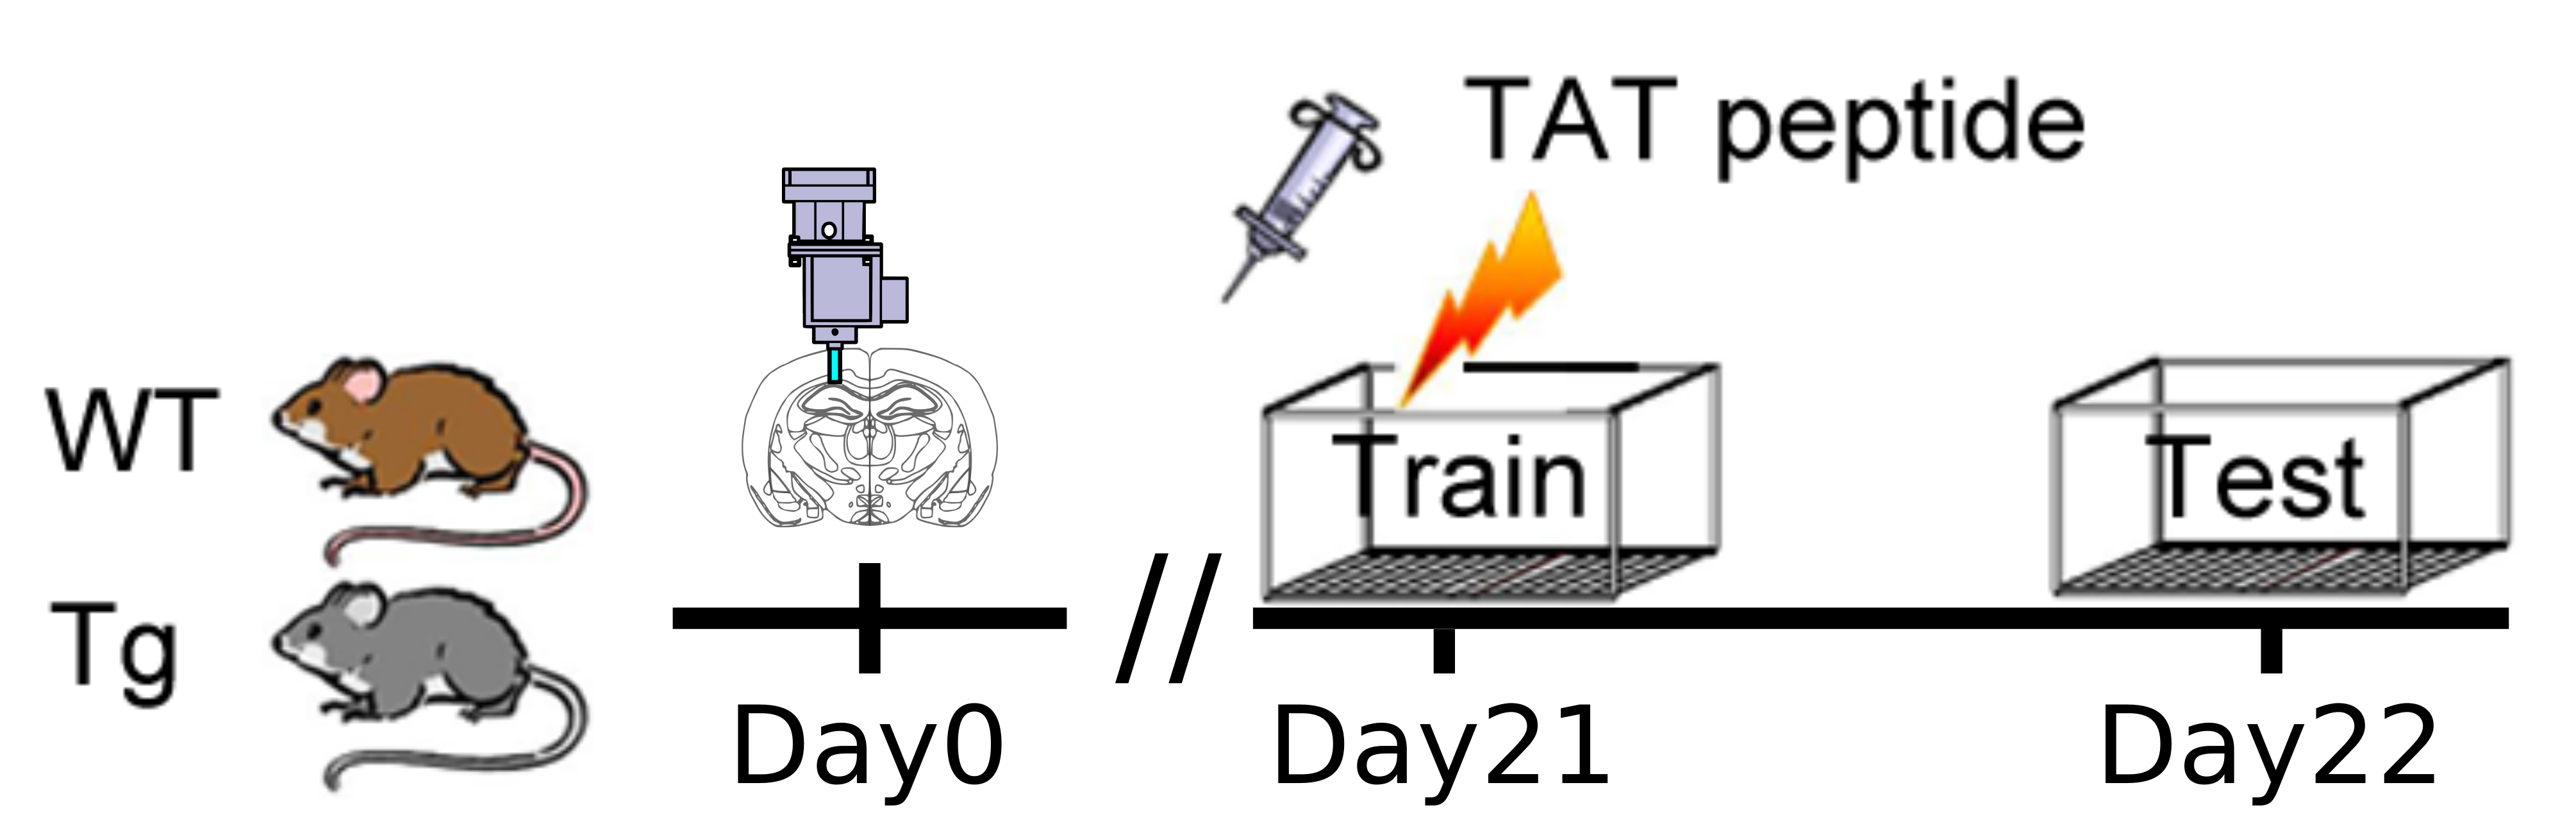
\includegraphics[width=\textwidth]{paradigm.png}
    \caption{Experimental paradigm. Adult \gls{wt} and \gls{tg} animals (with gCaMP6f expression) were implanted with a mini-microscope baseplate targeting CA1 hippocampus on day 0. The cells were visible three weeks later. Animals received \tglu peptide (i.p.) \SI{1}{\hour} before contextual fear conditioning. Animals were tested \SI{24}{\hour} later for freezing behaviour. Calcium activity were recorded for both training and testing session. \label{f.ad.paradigm}}
\end{figure}

\begin{figure}[h]
    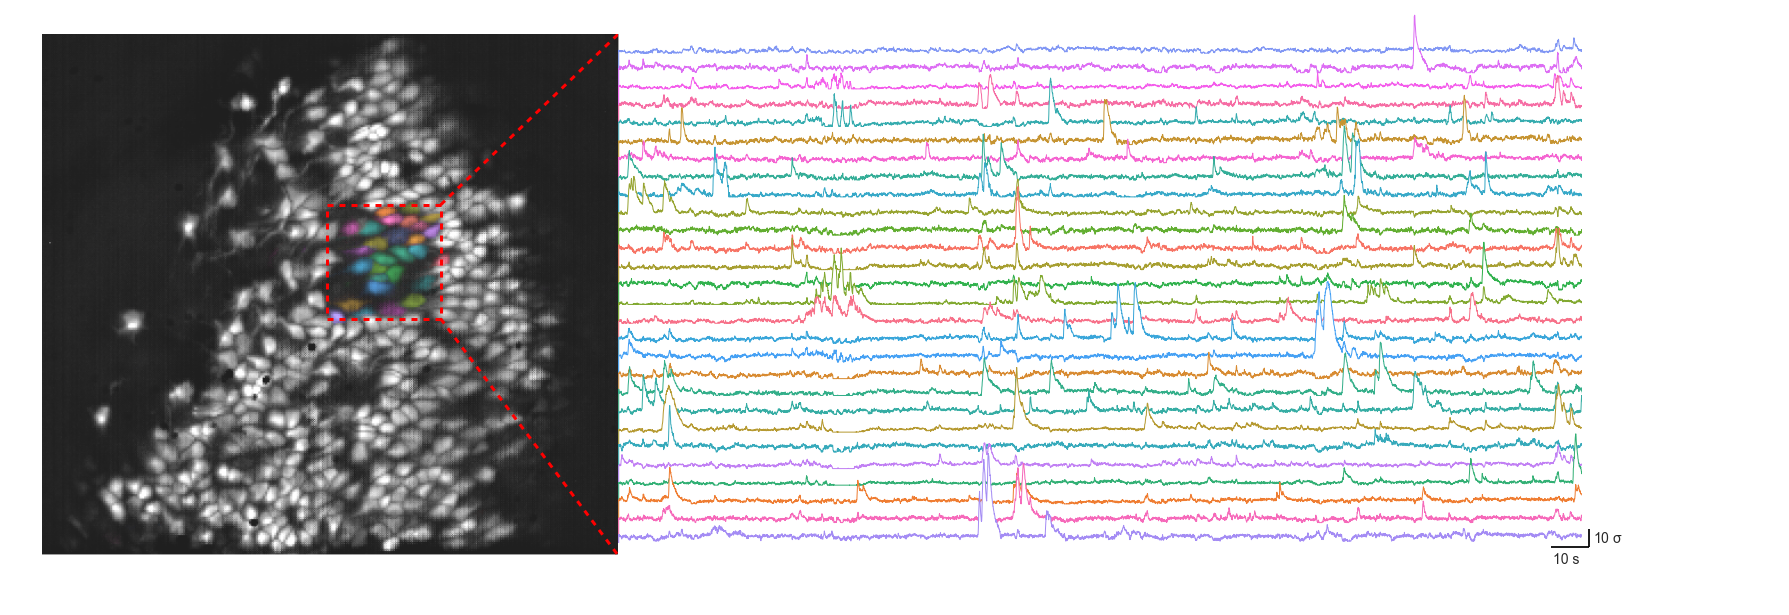
\includegraphics[width=\textwidth]{trace.png}
    \caption{Sample cell image and traces. Traces are random coloured and correspond to cells of the same colour. \label{f.ad.trace}}
\end{figure}


Figure~\ref{f.ad.freezing} shows the percent of freezing during testing. Two-way \gls{anova} has revealed significant main effect in genotype (F\tsb{1,27}=12.79, p=0.001) as well as a significant interaction between genotype and treatment (F\tsb{1,27}=5.45, p=0.027). Posthoc tests show that \gls{tg} animals have significant lower freezing (\gls{wt}-Veh vs \gls{tg}-Veh, T=4.21, p<0.001), and this effect is fully rescued by \tglu treatment (\gls{tg}-\glu vs \gls{tg}-Veh, T=2.85, p=0.008; \gls{wt}-Veh vs \gls{tg}-\glu, T=1.12, P=0.27). \tglu has no significant effect on \gls{wt} animals (\gls{wt}-Veh vs \gls{wt}-\glu, T=0.355, p=0.72). This result is consistent with our hypothesis, Tg animals showed decreased freezing, and this was rescued by \tglu treatment. 

\todo{freezing}
\begin{figure}[h]
    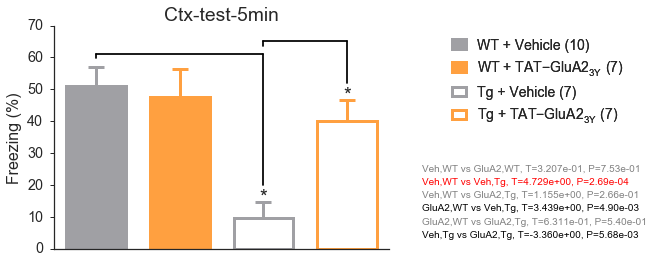
\includegraphics[width=\textwidth]{freezing.png}
    \caption{Percent of freezing during testing. \Gls{tg} animals have significant lower freezing, and \tglu treatment returns the freezing to wildtype level. \label{f.ad.freezing}}
\end{figure}



\subsection{\tglu rescues hyperactivity in \gls{tg} cells}

Figure~\ref{f.ad.acttrain} shows average cell activity during training session before footshock is delivered. During training, two-way \gls{anova} reveals significant major effects of genotype (F\tsb{1,3033}=6.2, p=0.01) and treatment (F\tsb{1,3033}=5.1, p=0.02) as well as a significant interaction between genotype and treament (F\tsb{1,3033}=7.7, p=0.006). Posthoc tests shows that \gls{tg}-Veh has significantly higher cell activity (WT-Veh vs Tg-Veh, T=-3.72, p<0.001), and \tglu treatment is able to restore average cell activity to \gls{wt} level. (Tg-\glu vs Tg-Veh, T=-3.58, p<0.001; WT-Veh vs Tg-\glu, T=0.14, p=0.89). \tglu does not have any effect on \gls{wt} animals (WT-Veh vs WT-\glu, T=-0.137, p=0.89) This result is consistent with previous reports in the literature \citep{verret12}, showing cells in Tg animals have increase overall cell activity. Interestingly, while \tglu treatment restores the the mean cell activity during training, the distribution of cell activity is significantly different from \gls{wt} (WT-Veh vs Tg-\glu, K=0.16, P<0.001). As is shown in the cumulative distribution plot, Tg-\glu still have a over-proportion of highly active cells. 
\todo{Discuss: \tglu is not able to rescue cells with very high activity}

Similar effect were found during testing (Figure~\ref{f.ad.acttest}). Two-way \gls{anova} revealled significant major effect of genotype (F\tsb{1,3029}=32.7, p<0.001) and treatment (F\tsb{1,3029}=27.4, p<0.001), as well as their interaction (F\tsb{1,3029}=78.4, p<0.001). Post-hoc tests show significant increase of cell activity in Tg-Veh group (WT-Veh vs Tg-Veh, T=-10.1, p<0.001), and this effect is corrected by \tglu treament (WT-Veh vs Tg-\glu, T=0.73, p=0.47; Tg-\glu vs Tg-Veh, T=-9.97, p<0.001). There is also a trend of increase in cell activity after \tglu treatment in \gls{wt} group, however the p-value is close to threshold after correction of multiple comparison (WT-Veh vs WT-\glu, T=-2.53, p=0.012, threshold = 0.013). Interestingly during testing, \tglu is able to fully rescue the hyper-activity in \gls{tg} group (\gls{kstest}: Veh-WT vs Tg-\glu, K=0.06, p=0.07; Tg-Veh vs Tg-\glu, K=2.29, p<0.001). These results suggest that the rescuing effect of \tglu in \gls{tg} animals is slow and long-lasting.

\begin{figure}[h]
    \begin{subfigure}[h]{\textwidth}
        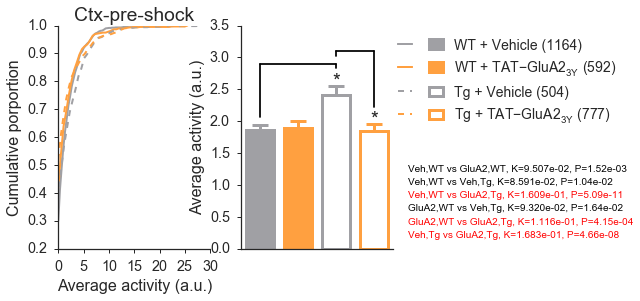
\includegraphics[width=\textwidth]{activity_train.png}
        \caption{\label{f.ad.acttrain}}
    \end{subfigure}
    \begin{subfigure}[h]{\textwidth}
        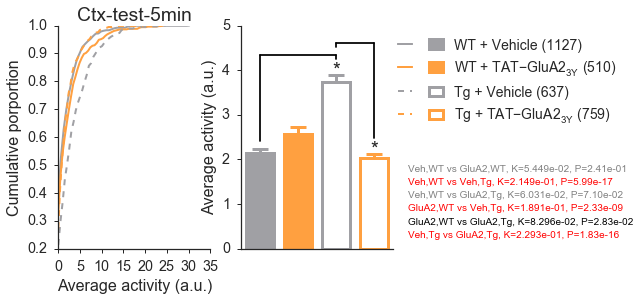
\includegraphics[width=\textwidth]{activity_test.png}
        \caption{\label{f.ad.acttest}}
    \end{subfigure}
    \caption{Distribution and mean of average cell activity during \subref{f.ad.acttrain} training and \subref{f.ad.acttest} testing. Cells in the Tg animals are significantly more active, and this is rescued by \tglu treatment. \label{f.ad.activity}}
\end{figure}

\subsection{\tglu rescues freezing encoding deficit in \gls{tg} cells}

We then investigated that how \gls{wt} and \gls{tg} cells encodes freezing. First we looked at cells individually, and calculated the mutual information between cell firing and freezing \citep{ross14, victor02}. This measurement reflects how much prediction power a cell has for freezing in a period of time. The group differences in freezing information is then compared using two-way \gls{anova}. There is significant main effect in both genotype (F\tsb{1,4380}=254.0, p<0.001) and treatment (F\tsb{1,4380}=54.7, p<0.001), and a significant interaction between the two factors (F\tsb{1,4380}=126.7, p<0.001). Posthoc tests show Tg-Veh group has significantly less freezing information (WT-Veh vs Tg-Veh, T=19.3, p<0.001), and this deficit is partially rescued by \tglu treatment (Tg-\glu vs Tg-Veh, T=13.2, p<0.001), as Tg-\glu group has significantly less freezing information than WT-Veh group (WT-Veh vs Tg-\glu, T=6.0, p<0.001; Figure~\ref{f.ad.freeze_info}). WT-\glu has significantly less freezing information than WT-Veh, although the significance is close to threshold (WT-Veh vs WT-\glu, T=2.5, p=0.011, threshold=0.125). This result suggests in the \gls{tg} group, the cell activity in hippocampus \gls{ca1} does not predict the animal's behaviour well, however this is improved with \tglu treatment but not fully rescued. 
\begin{figure}[h]
    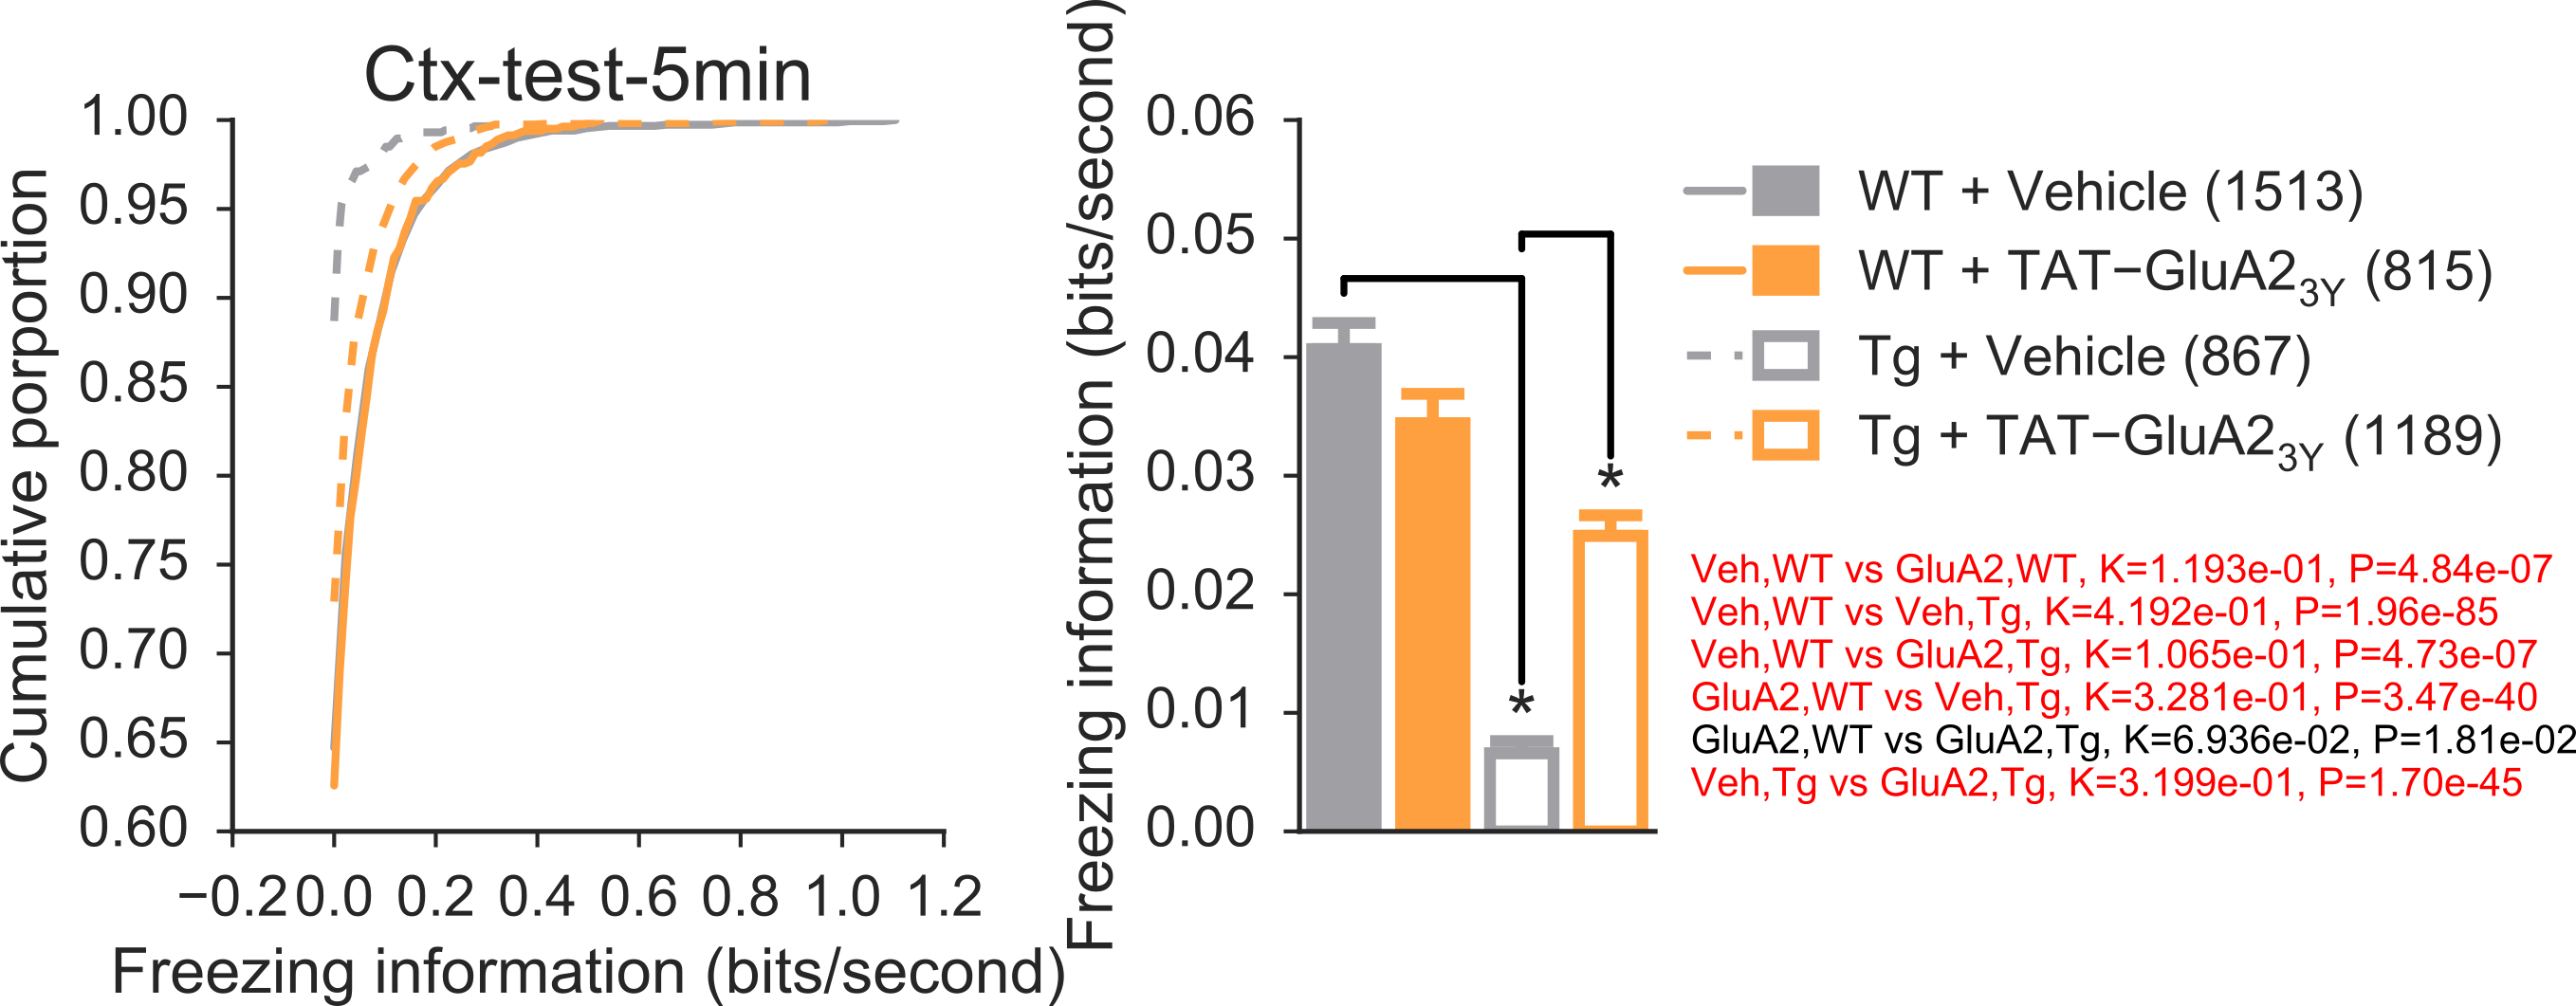
\includegraphics[width=\textwidth]{freeze_info.png}
    \caption{Freezing information during testing. This measurement represent how much information a cell have in a period of time about whether the animal is freezing. Cells in \gls{tg} animals encode significantly less freezing than the \gls{wt} groups, and \tglu treatment can only partially rescue the effect. \label{f.ad.freeze_info}}
\end{figure}
    

While all the measurements we have performed considers each cell individually, are the cells independent of each other, or is part of the information encoded in the coordination between them? To answer this question, we have build two classifiers: a \gls{nbc} which models the cells independent of each other, and a \gls{gsvm}, which also uses the dependency between cells for prediction. The result is shown in Figure~\ref{f.ad.classifier}. 

A three-way \gls{anova} of genotype $\times$ treatment $\times$ classifier was carried out. There are significant main effect of genotype (F\tsb{1,50}=15.6, p<0.001), treatment (F\tsb{1,50}=5.5, p=0.02) and classifier (F\tsb{1,50}=9.0, p=0.004). There is also a significant interaction between genotype and treatment (F\tsb{1,50}=14.2, p<0.001), and no significant interactions involving the classifier factor. Since the classifier factor only have a significant major effect, for the posthoc tests we used F-test to only compare different levels of genotype and treatment. F1 score of Tg-Veh is significantly less than WT-Veh (F\tsb{2,50}=16.4, p<0.001), and this effect is rescued by \tglu treatment (Tg-\glu vs Tg-Veh, F\tsb{2,50}=9.7, p<0.001). There is no significant difference between WT-Veh and Tg-\glu (F\tsb{2,50}=0.63, p=0.54), and \tglu treatment has no significant effect on \gls{wt} group (WT-Veh vs WT-\glu, F\tsb{2,50}=0.20, p=0.81).  

These results show \gls{gsvm} significantly outperforms the \gls{nbc} classifier across all groups, suggesting that the network encodes more information than the cells individually. Moreover, both classifiers perform significantly worse in the \gls{tg} group, further supports our hypothesis that \gls{tg} animals have inferior fear memory encoding. Moreover, this deficit is fully rescued by \tglu treatment.

\begin{figure}[h]
    \begin{subfigure}[h]{\textwidth}
        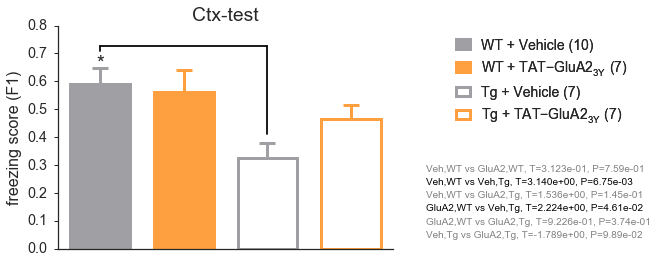
\includegraphics[width=\textwidth]{nb.png}
        \caption{\label{f.ad.nb}}
    \end{subfigure}
    \begin{subfigure}[h]{\textwidth}
        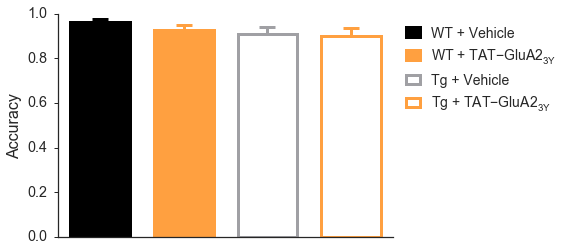
\includegraphics[width=\textwidth]{svm.png}
        \caption{\label{f.ad.svm}}
    \end{subfigure}
    \caption{Performance of \subref{f.ad.nb} \gls{nbc} and \subref{f.ad.svm} \gls{gsvm} in predicting freezing from cell activity. Results are measured as F1 score. Both classifiers showed inferior performance in \gls{tg} group, further supports the hypothesis that \gls{tg} animals have sub-optimal freezing encoding. Interestingly, since \gls{nbc} assumes the cells are independent and \gls{gsvm} is more general, the performance difference between the two suggest a portion of freezing information is encoded in the coordination between the activity of the cells. \label{f.ad.classifier}}
\end{figure}




\subsection{Difference of encoding in \gls{tg} animals is not a result of animal's behaviour}

However, given that the Tg animals also show behavioural difference, we then try to answer the question: is the difference in neural coding inherit of the Alzheimer animal, or a result of the different behaviour? Given that CA1 cells are known to represent place, we have calculated the freezing information marginalized over all animal positions, therefore eliminating it's effect in the calculation of freezing information. Two-way \gls{anova} shows significant main effects in genotype (F\tsb{1,4380}=241.3, p<0.001) and treatment (F\tsb{1,4380}=147.4, p<0.001), as well as significant interaction between the two factors (F\tsb{1,4380}=126.7, p<0.001). Posthoc tests show that Tg-Veh has significant lower freezing information with position controlled (WT-Veh vs Tg-Veh, T=19.0, p<0.001), and fully rescued by \tglu (Tg-\glu vs Tg-Veh, t=16.5, p<0.001; WT-Veh vs Tg-\glu, t=1.9, p=0.06, threshold=0.0125). The result is similar and shown in Figure~\ref{f.ad.freeze_ctrl}.  
\begin{figure}[h]
    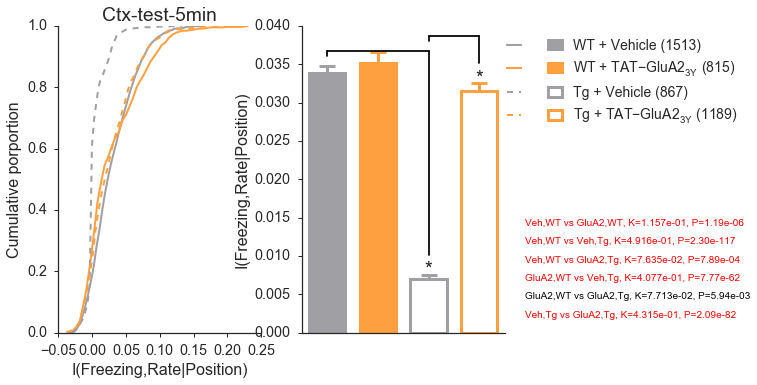
\includegraphics[width=\textwidth]{freeze_position.png}
    \caption{Freezing information conditioned on animal's position. This measurement removes the effect of position from freezing information measurement. This result is similar to Figure~\ref{f.ad.freeze_info}. This suggest that the position of the animal is not a confounding factor for freezing information measurement. \label{f.ad.freeze_ctrl}}
\end{figure}


An additional potential confound comes from the animal's behaviour. Within \gls{wt} animals, there is a significant correlation between freezing information and freezing \todo{stats and figure}. Given that \gls{tg} animals do not freeze well during testing, we ask is the encoding deficit found in \gls{tg} animals explained by the correlation of freezing and encoding? To investigate this question, we added freezing as a covariate into the two-way \gls{anova} model for position-controlled freezing information. The resulting model shows while percent of freezing is a significant confound in measuring freezing information (F\tsb{1,4379}=42.0, p<0.001), there is still significant major effect of genotype (F\tsb{1,4379}=34.0, p<0.001) and treatment (F\tsb{1,4379}=6.7, p=0.009), as well as a significant interaction between the two factors (F\tsb{1,4379}=5.6, p=0.017). Similarly to Figure~\ref{f.ad.freeze_ctrl}, Posthoc tests have found a significant decrease of freezing information in Tg-Veh with freezing level controlled (WT-Veh vs Tg-Veh, t=5.46, p<0.001), as well as a partial rescue by \tglu treatment (Tg-\glu vs Tg-Veh, t=3.45, p=0.001; WT-Veh vs Tg-\glu, t=2.93, p=0.003). And again, no effect of \tglu on \gls{wt} animals (WT-Veh vs WT-\glu, t=-0.30, p=0.75). These results suggest that while freezing information is correlated with percent of freezing, \gls{tg} animals have additional deficit in encoding freezing, and this deficit is partially rescued by \tglu treatment. 

\begin{comment}
In addition, we also checked whether the freezing information coding is a result of different freezing or uneven spatial coverage of the behavioural chamber, which are represented by freezing entropy and spatial entropy respectively. To check these two factors, we have pooled the groups with similar behaviour (\gls{wt}, \gls{wt}-\tglu, \gls{tg}-\tglu), and correlated percent freezing, freezing entropy, total distance and spatial entropy against freezing information within the pooled groups. If the behavioural measurement have no influence in the freezing information, we would expect no correlation. Indeed, that is what we have found in Figure~\ref{f.ad.corrs}. These control measurements have shown that the reduction of freezing encoding in the Tg animals is not affected by the difference in the animals' behaviour.
\begin{figure}[h]
    \begin{subfigure}[t]{.5\textwidth}
        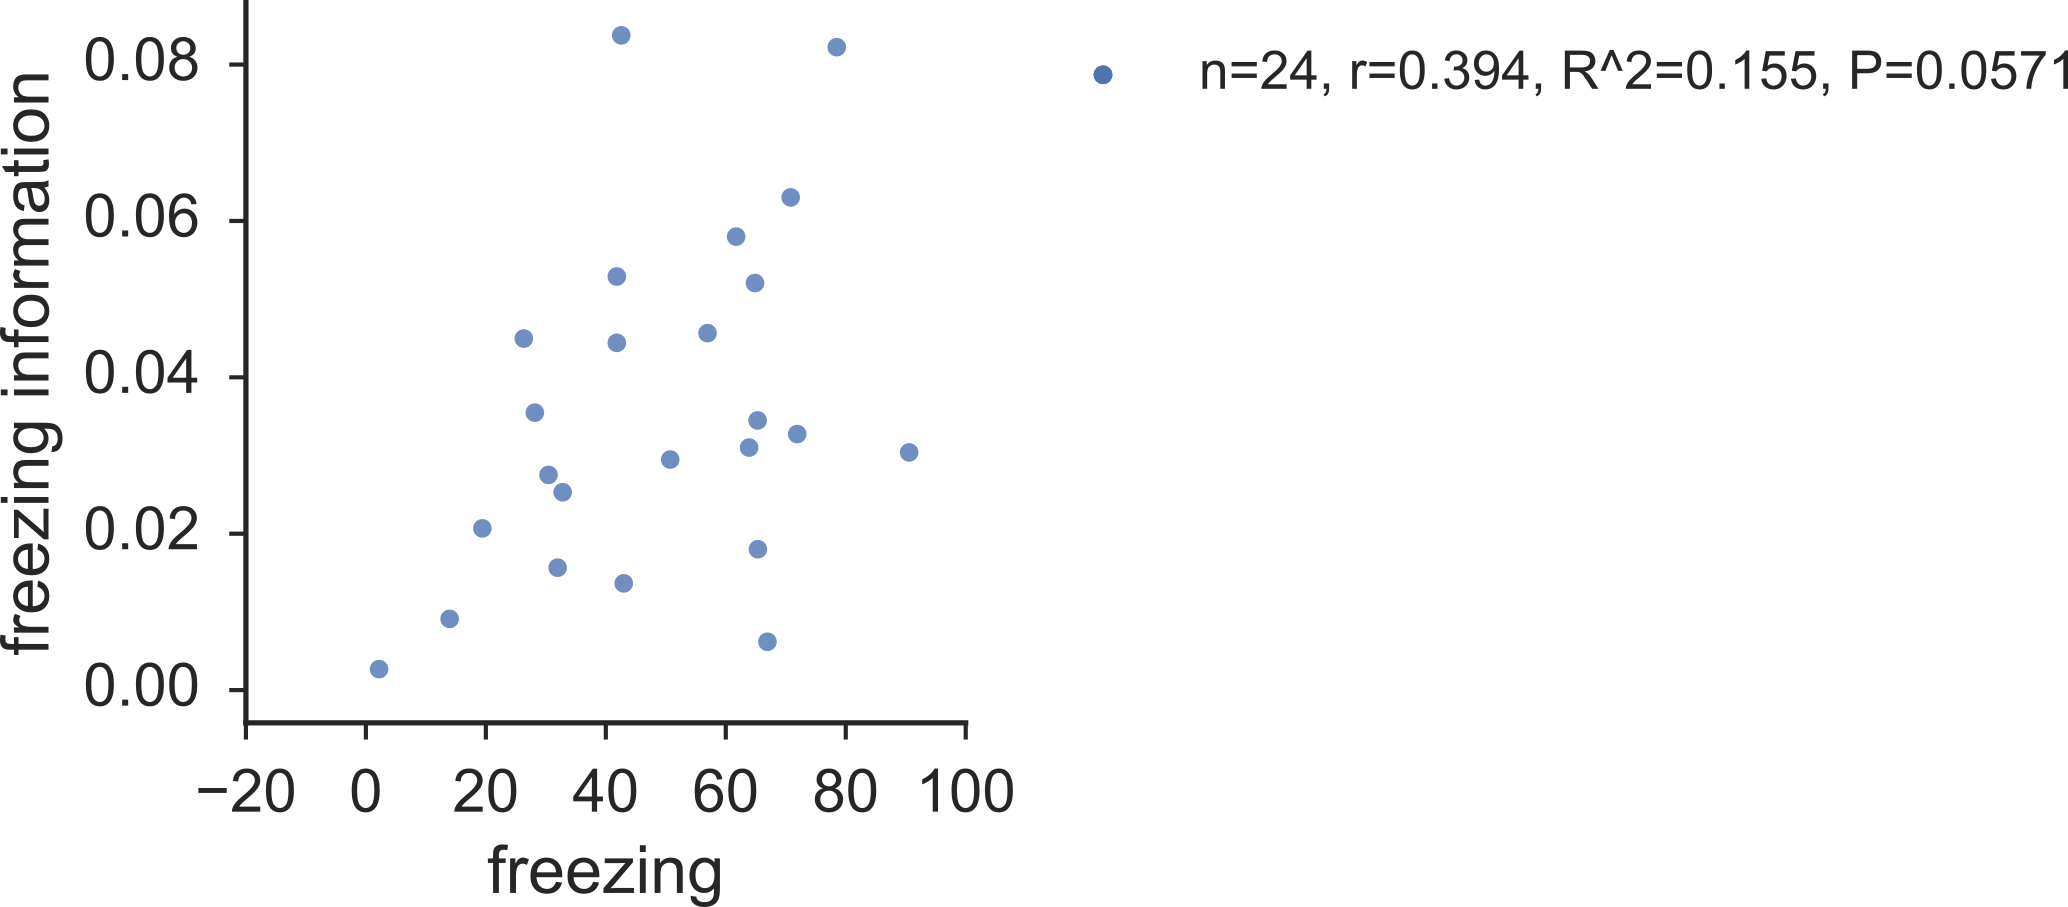
\includegraphics[width=\textwidth]{corr1.png}
        \caption{}
    \end{subfigure}
    \begin{subfigure}[t]{.5\textwidth}
        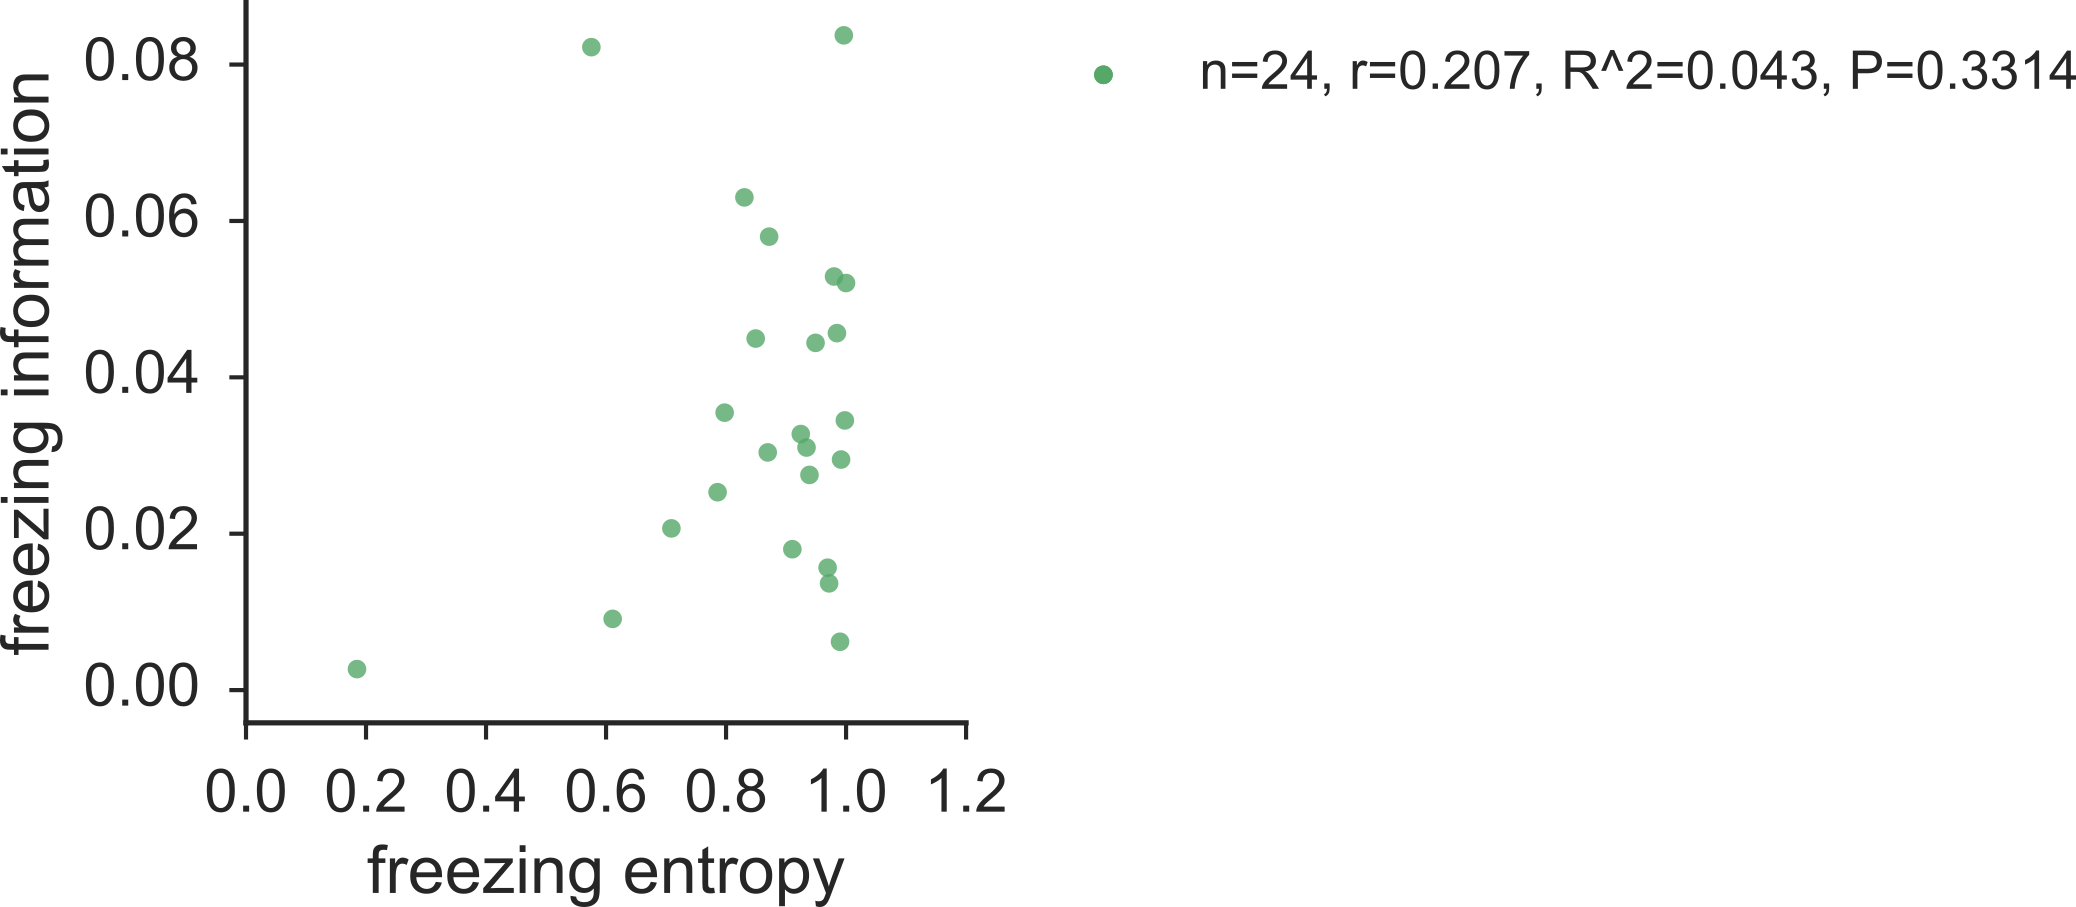
\includegraphics[width=\textwidth]{corr2.png}
        \caption{}
    \end{subfigure}
    \begin{subfigure}[t]{.5\textwidth}
        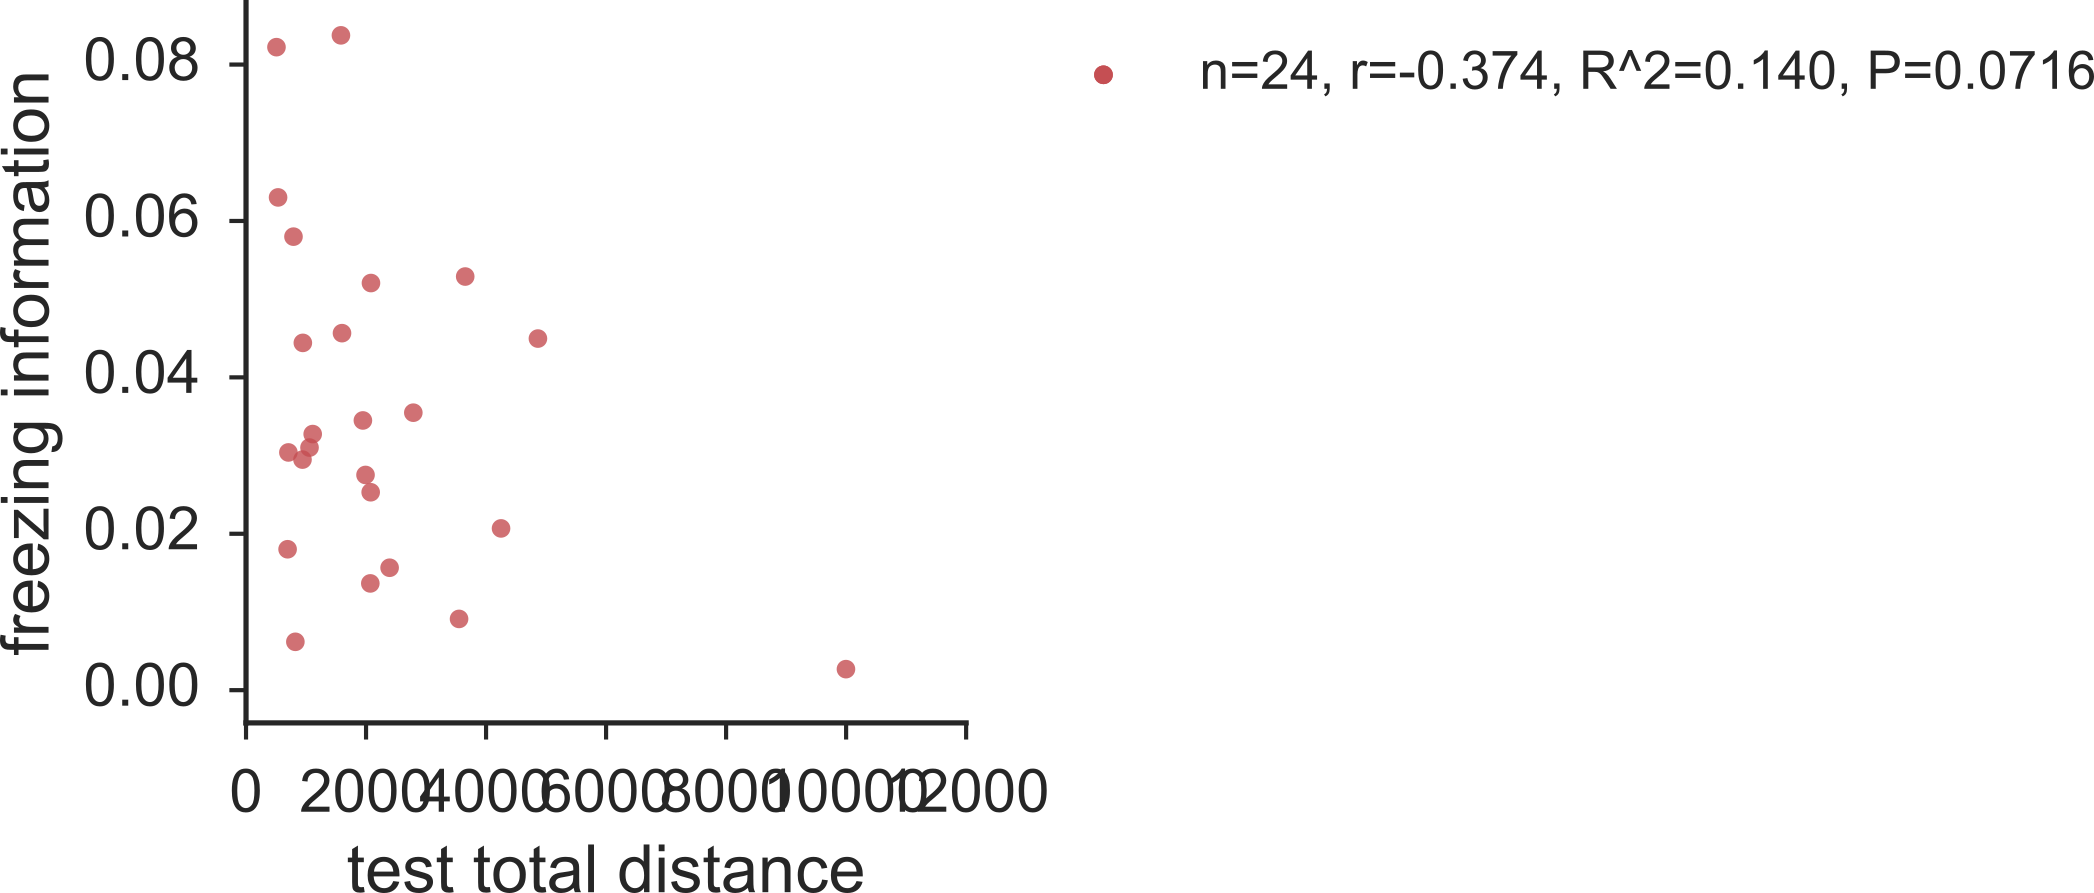
\includegraphics[width=\textwidth]{corr3.png}
        \caption{}
    \end{subfigure}
    \begin{subfigure}[t]{.5\textwidth}
        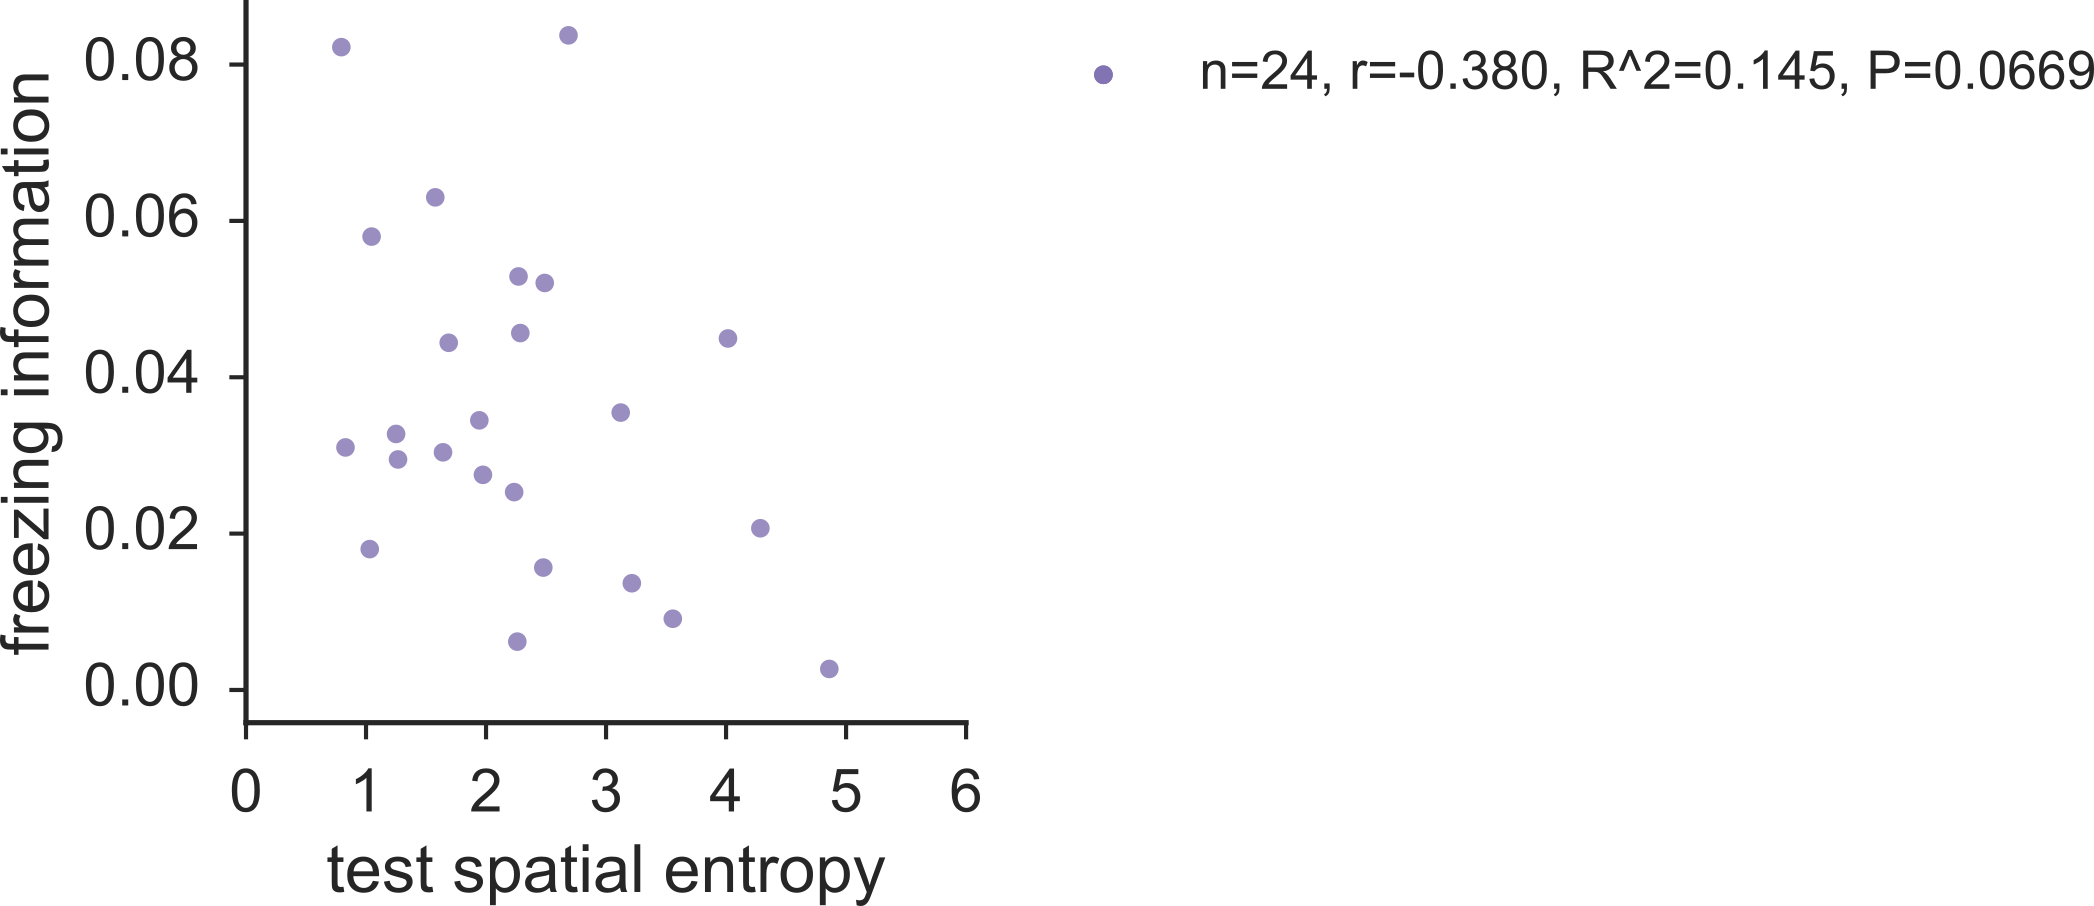
\includegraphics[width=\textwidth]{corr4.png}
        \caption{}
    \end{subfigure}
    \caption{Scatter plots of varies behaviour measurement against freezing information, in pooled \gls{wt}, \gls{wt}-\glu and \gls{tg}-\glu. Given there is no group difference between the three groups, if any of the behaviour factor is confounding, the it will contribute to within-group difference and correlate with freezing information. We have found no significant correlations. However the near significance of percent freezing and spatial entropy correlations will need further investigation. \label{f.ad.corrs}}
\end{figure}
\end{comment}


\subsection{\tglu rescues recall by decreasing activity}

The next question we investigated is, if the cells are encoding freezing, how do they encode? In figure~\ref{f.ad.ch_activity} we selected all the cells that have more than 0.01 bits/second (which amounts to ~40\% in the normal groups and 10\% of the cells in the \gls{tg} group), and plotted the difference of average activity when the animal is freezing and not freezing. Interestingly, the majority of the cells encode freezing by decreasing their activity. This can also be seen representatively in the sample trace (Figure~\ref{f.ad.sample_trace}).
\begin{figure}[h]
    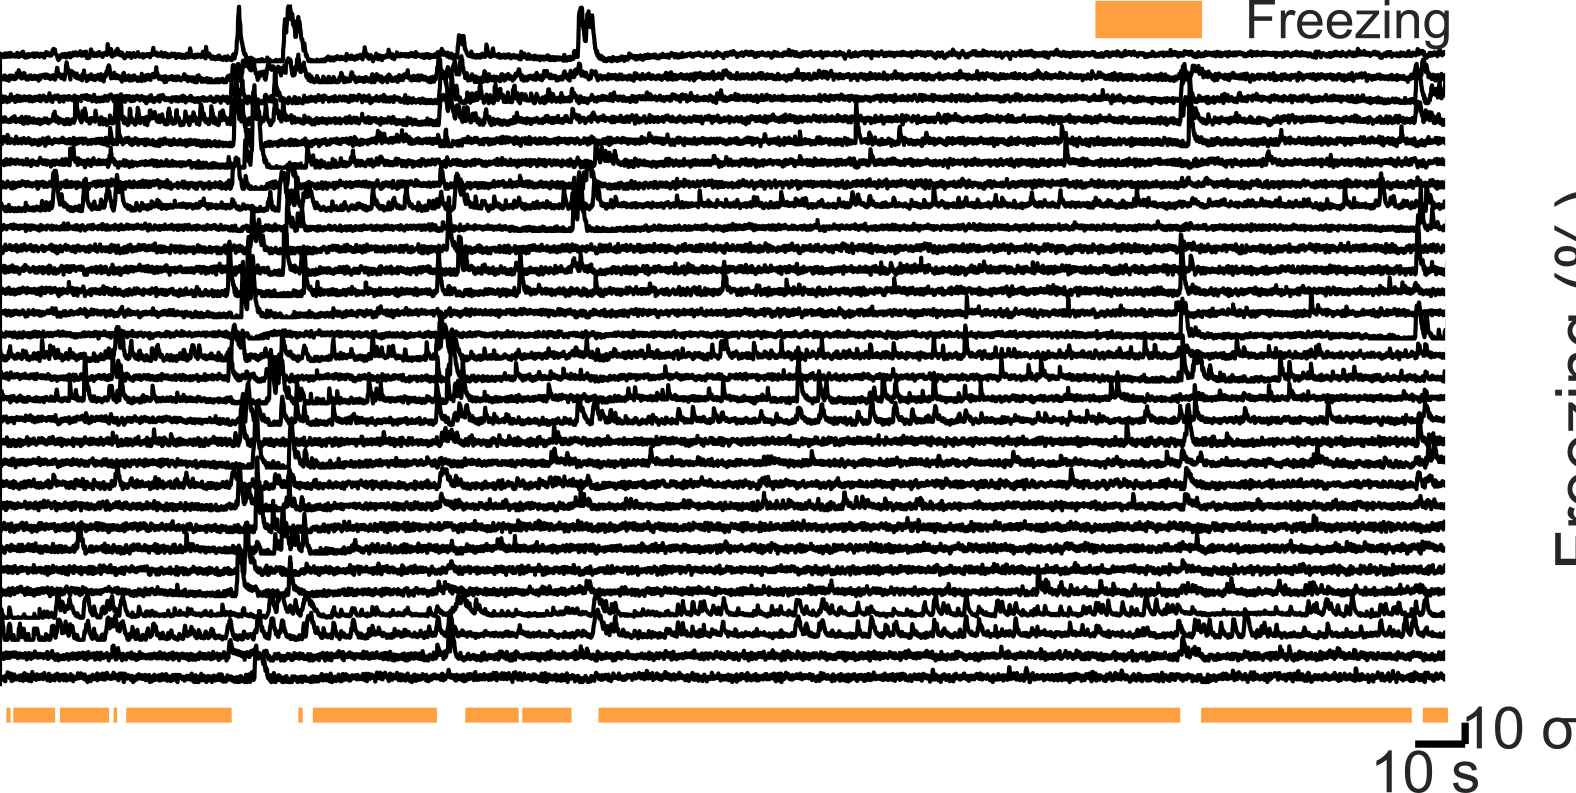
\includegraphics[width=\textwidth]{sample_trace.png}
    \caption{Sample traces from cells with highest freezing information in an animal. It appears that cells encode freezing by decreasing their activity. \label{f.ad.sample_trace}}
\end{figure}
\begin{figure}[h]
    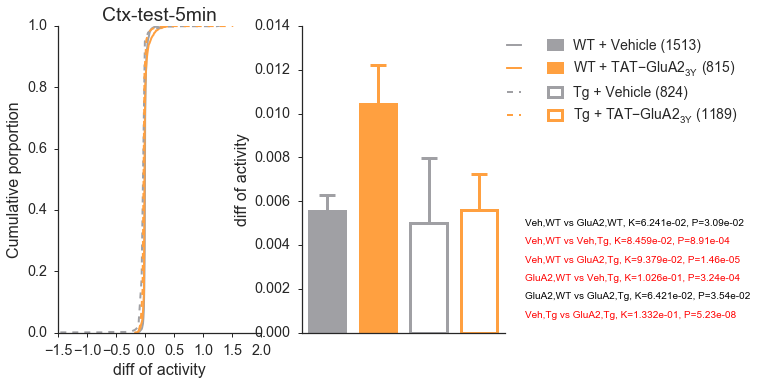
\includegraphics[width=\textwidth]{ch_activity.png}
    \caption{Distribution and mean of activity difference between freezing and none-freezing, in cell with freezing information more than 0.01. This confirms the intuition from Figure~\ref{f.ad.sample_trace} that most of the cells encode freezing by decreasing activity. \label{f.ad.ch_activity}}
\end{figure}

Given the cells tend to have decreased activity during freezing, we also examined the average cell activity when the animal is freezing, and activity when the animal is not (Figure~\ref{f.ad.activity_freezing}). Two-way \gls{anova} on the average activity when animals are freezing shows significant main effect in genotype (F\tsb{1,3034}=6.9, p=0.008) and treatment (F\tsb{1,3034}=18.7, p<0.001). The interaction between them is not significant (F\tsb{1,3034}=-0.03, p=0.97). \Gls{tg} animals show significantly increased activity during freezing, and \tglu treatment has a significant inhibitory effect on cell activity. \todo{discuss about highly active cells in the cumulative distribution plot}

Two-way \gls{anova} revealed a significant effect of treatment (F\tsb{1,3029}=12.3, p<0.001) and a significant genotype $\times$ treatment interaction (F\tsb{1,3029}=13.6, p<0.001). \tglu treatment only significantly decreased activity in the \gls{tg} animals (Tg-\glu vs Tg-Veh, T=-5.4, p<0.001). These results suggest the \tglu{} may rescue the \gls{tg} phenotype by globally decrease background cell activity.
\begin{figure}[h]
    \begin{subfigure}[h]{\textwidth}
        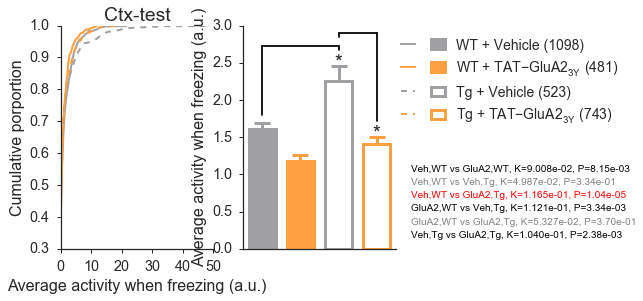
\includegraphics[width=\textwidth]{activity_freezing.png}
        \caption{\label{f.ad.actf}}
    \end{subfigure}
    \begin{subfigure}[h]{\textwidth}
        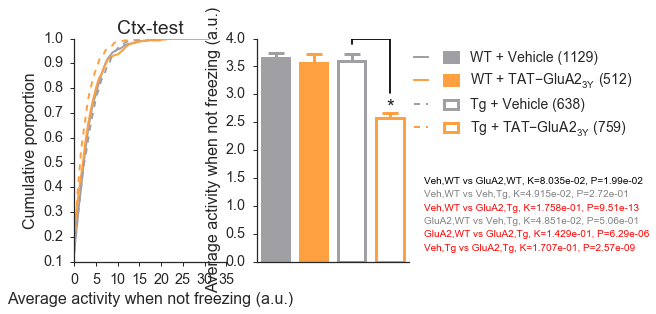
\includegraphics[width=\textwidth]{activity_moving.png}
        \caption{\label{f.ad.actnf}}
    \end{subfigure}
    \caption{Average cell activity during \subref{f.ad.actf} freezing and \subref{f.ad.actnf} not freezing. Cells in \gls{tg} animals have significantly higher activity during freezing, suggesting a sub-optimal encoding of freezing. Interestingly, \tglu also showed a decreased activity when the animal is not freezing, suggesting that the effect of \tglu maybe a global decrease of cell activity. \label{f.ad.activity_freezing}}
\end{figure}

\subsection{Freezing encoding precedes freezing behaviour}



\begin{figure}[h]
    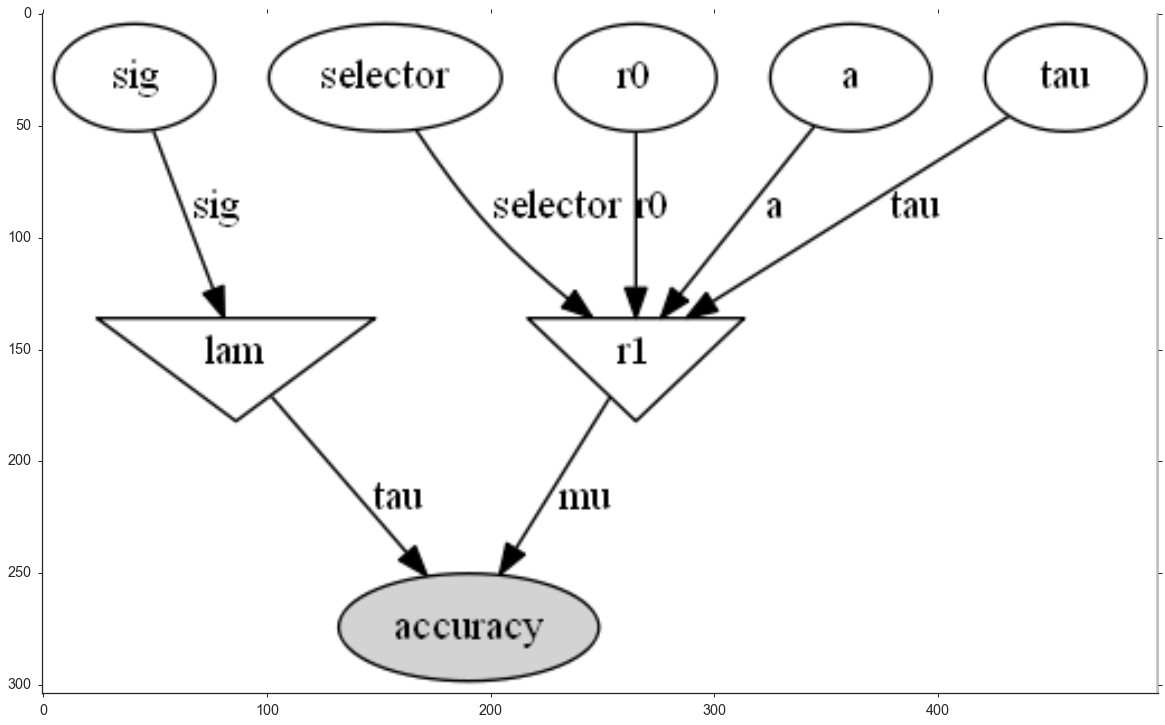
\includegraphics[width=\textwidth]{bayes_model.png}
    \caption{Bayes model for change point detection. The accuracy is modelled as a gaussian distribution with mean as a function of time and constant variance. In the null hypothesis, the mean is constant and estimated from the data. In the alternative hypothesis, the mean is modeled as constant up to the change point, then as a linear function of time with a negative slope. A Bernoulli variable $selector$ is estimated to choose from each of the hypothesis. \label{f.ad.bayesmodel}}
\end{figure}\todo{bayes model}

To examine whether the freezing encoding is an artifact of the freezing behaviour, we plotted average prediction accuracy for the classifiers at the time animals behaviour transits into freezing. We used Bayes modelling (Figure \ref{f.ad.bayesmodel}) to detect and compare whether the prediction accuracy changes before behaviour change.  

The result is summarized in Figure~\ref{f.ad.into_f}. In the \gls{nbc}, we have found very strong evidence for a change point in every group (all Bayes factors BF10 > \num{5e4}). The change point appears $3.4_{-0.1}^{+0.1}$\SI{}{\s} in WT-Veh, $2.8_{-0.1}^{+0.1}$\SI{}{\second} in WT-\glu, $2.8_{-0.3}^{+0.2}$\SI{}{\second} in Tg-Veh, and $2.6_{-0.1}^{+0.1}$\SI{}{\second} in Tg-\glu before freezing onset (uncertainties are \SI{95}{\percent} credible intervals). Pairwise comparisons show very strong evidence that the change point in WT-Veh occurs earlier, while the other three groups occur at the same time (WT-Veh vs WT-\glu, BF10 > \num{250}; WT-Veh vs Tg-Veh, BF10 = \num{7.5}; WT-Veh vs Tg-\glu, BF10 > \num{250}; all other comparisons BF10 < \num{0.2}). Since \gls{nbc} regards each cell independently, this result suggest that the freezing signal in individual cells occurs earlier than the onset of freezing behaviour.

On the other hand in the \gls{gsvm}, we have found very strong evidence for change point in WT-Veh (BF10 > \num{5e4}), WT-\glu (BF10 > \num{5e4}) and Tg-\glu (BF10 > \num{5e4}), and also strong evidence that a change point does not present in Tg-Veh (BF10 < \num{0.02}). The change points are estimated to be $0.6_{-0.1}^{+0.0}$\SI{}{\s} in WT-Veh, $2.6_{-0.3}^{0.2}$\SI{}{\second} in WT-\glu, and $0.3_{-0.2}^{+0.1}$\SI{}{\s} in Tg-\glu, before the freezing onset. Pairwise comparisons show very strong evidence of a earlier change point in WT-\glu than the other groups (WT-\glu vs WT-Veh, BF10 > \num{250}; WT-\glu vs Tg-\glu, BF10 > \num{250}). There is minimal evidence that the change point in WT-Veh is earlier than Tg-\glu (BF10 = \num{2.5}). These results suggest that the freezing signal in the network occur earlier than freezing behaviour in \gls{wt} groups, however not present in the \gls{tg} group. \tglu treatment of the \gls{tg} animals is able to partially rescues this effect. In addition, the network freezing signal occur earlier in WT-\glu than the other groups.

\begin{figure}[h]
    \begin{subfigure}[h]{\textwidth}
        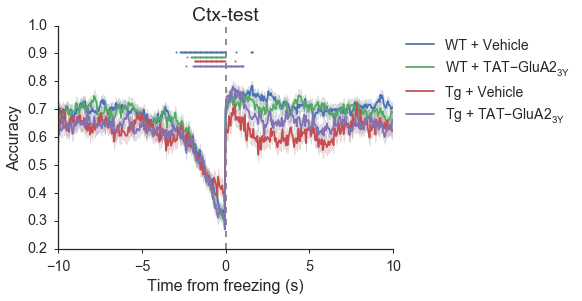
\includegraphics[width=\textwidth]{nb_into_freezing.png}
        \caption{\label{f.ad.nb_into_f}}
    \end{subfigure}
    \begin{subfigure}[h]{\textwidth}
        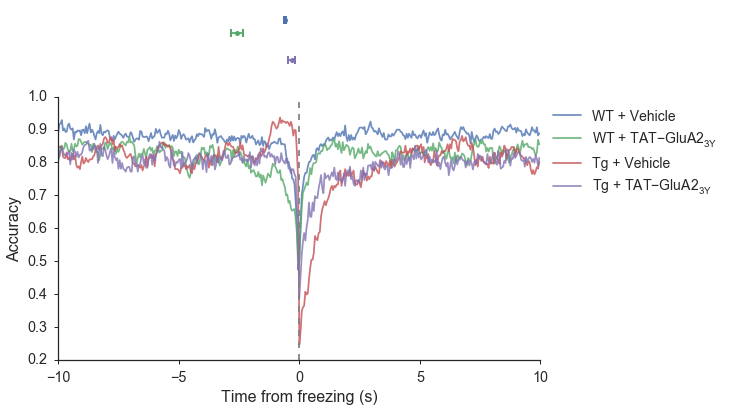
\includegraphics[width=\textwidth]{svm_into_freezing.png}
        \caption{\label{f.ad.svm_into_f}}
    \end{subfigure}
    \caption{Average accuracy of classifiers at the beginning of freezing behaviour. For \gls{wt} and \gls{tg}-\glu groups, both \gls{nbc} and \gls{gsvm} shows significant lower performance just before the animals show freezing behaviour. This suggests that \gls{ca1} neural activity precedes behaviour. The errorbars on the top shows \SI{95}{\percent} credible interval of the change point, if the alternative hypothesis is favoured. \label{f.ad.into_f}}
\end{figure}


\subsection{\Gls{tg} animals can initiate freezing}
We then investigated whether the deficits in \gls{tg} mice is due to less freezing initiation or freezing maintanence. Figure~\ref{f.ad.freezing_profile} summarizes the number and length of freezing periods in each group. There is no significant difference between groups in the number of freezing periods (Figure~\ref{f.ad.freezing_freq}, omnibus F\tsb{3,27}=0.84, p=0.48). On the length of freezing periods, there is significant main effect of genotype (F\tsb{1,27}=17.7, p<0.001), and a significant interaction between genotype and treatment (F\tsb{1,27}=6.5, p=0.01). Poshhoc tests shows Tg-Veh mice have significantly shorter freezing periods (WT-Veh vs Tg-Veh, T=4.75, p<0.001), and this deficit is fully rescued by \tglu treatment (Tg-\glu vs Tg-Veh, T=3.10, p=0.002; WT-Veh vs Tg-\glu, T=1.66, p=0.10). There is no effect of \tglu on \gls{wt} mice (T=0.22, p=0.83). 

\begin{figure}[h]
    \begin{subfigure}[h]{\textwidth}
        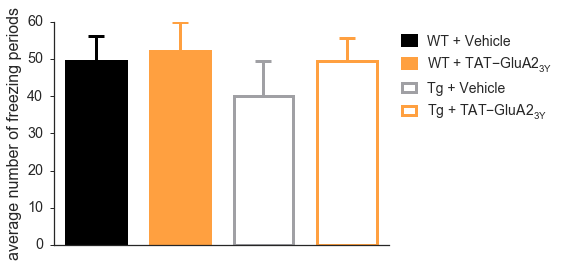
\includegraphics[width=\textwidth]{freezing_frequency.png}
        \caption{\label{f.ad.freezing_freq}}
    \end{subfigure}
    \begin{subfigure}[h]{\textwidth}
        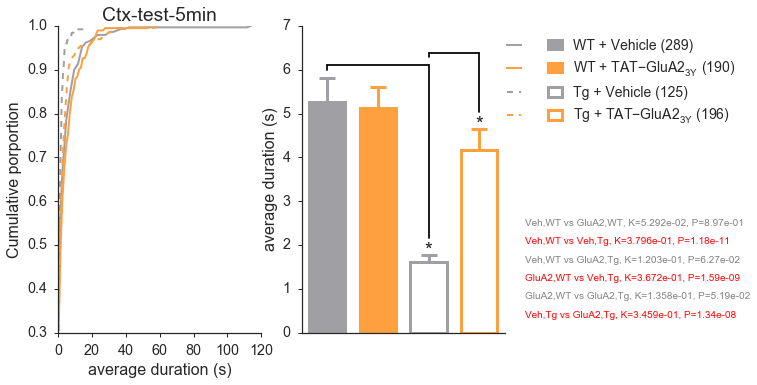
\includegraphics[width=\textwidth]{freezing_length.png}
        \caption{\label{f.ad.freezing_length}}
    \end{subfigure}
    \caption{Average number of freezing periods (\subref{f.ad.freezing_freq}) and length of freezing periods (\subref{f.ad.freezing_length}). \Gls{tg} mice freeze as often as \gls{wt} mice, but with less duration. This is rescued by \tglu treatment. \label{f.ad.freezing_profile}}
\end{figure}




\subsection{\Gls{tg} animals have deficits recall freezing memory}
Given that \gls{tg} animals can initiate freezing behaviour, we suspect that their memory deficits is due to memory recall rather than memory encoding. To test this hypothesis, we trained the animals without \tglu, and \SI{3}{\day} later, treat the animal with \tglu or saline vehicle when they are shortly exposed to the training context as a reminder. The memory test occured \SI{24}{\hour} later. The result is summarized in Figure~\ref{f.ad.reminder1}. We found a significant interaction between genotype and treatment (\todo{stats}). Post-hoc tests shows Tg-Veh has a significant memory deficit (\todo{stats}), however this effect is fully rescued by \tglu treatment (\todo{stats}). This result suggests that \gls{tg} animals have intact memory encoding and deficits in memory recall. The recall deficit can be rescued with \tglu treament if the animal is exposed to a reminder.

\begin{figure}[h]
    \begin{subfigure}[h]{\textwidth}
        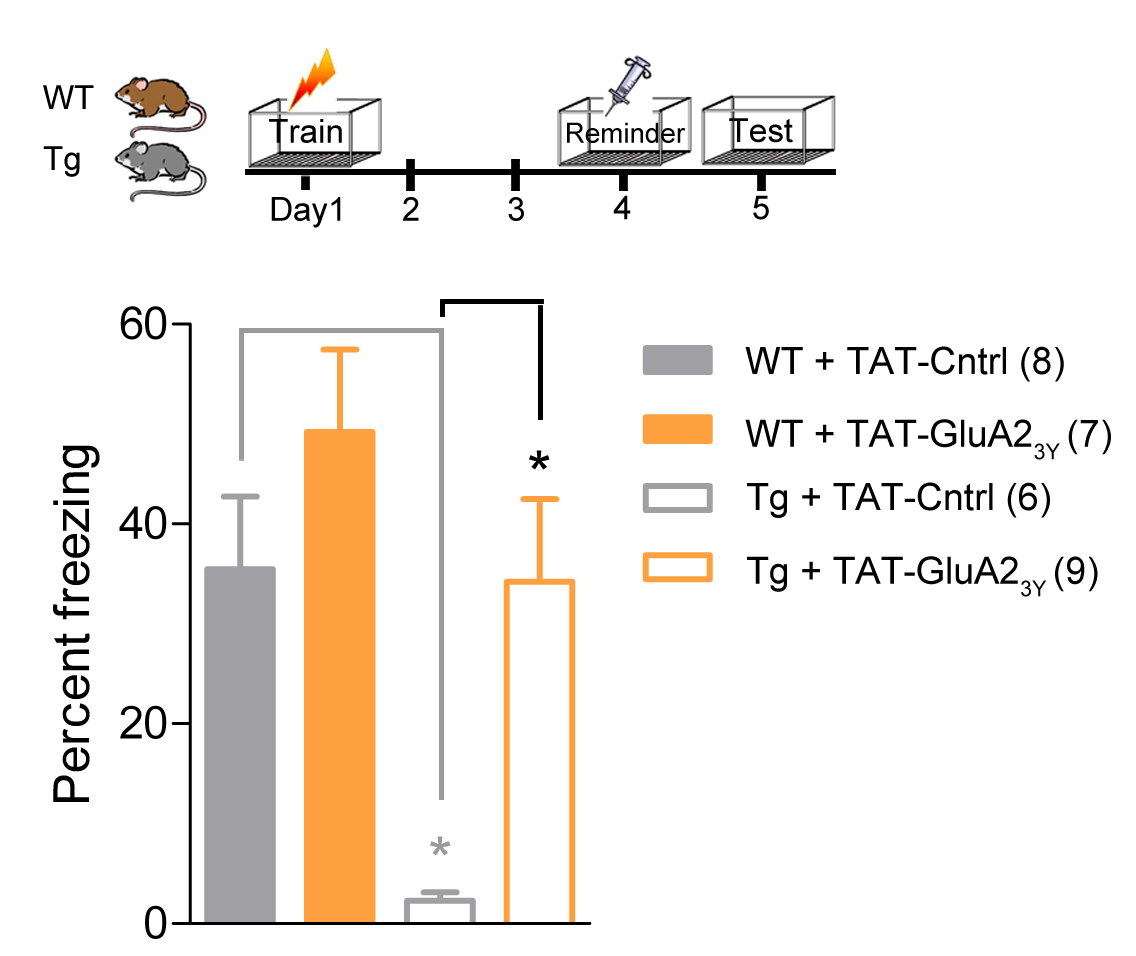
\includegraphics[width=\textwidth]{reminder1.png}
        \caption{\label{f.ad.actf}}
    \end{subfigure}
    \caption{ \label{f.ad.reminder1}}
\end{figure}

We then investigated whether the effect of the \tglu is memory specific. In a separate cohort of animals, we use a similar protocol as Figure~\ref{f.ad.reminder1}, except the animals received \tglu in their homecage instead of the reminder (Figure~\ref{f.ad.reminder2}). In this case, the \tglu treatment does not have any effect on memory recall. There is a significant main effect of genotype (\todo{stats}), and the genotype $times$ treatment interaction is not significant (\todo{stats}; Figure~\ref{f.ad.reminder2}). Together, these two pieces of results suggest that \gls{tg} animals have normal memory encoding but unable to recall, and \tglu rescues the deficit only when the memory is reminded.


\begin{figure}[h]
    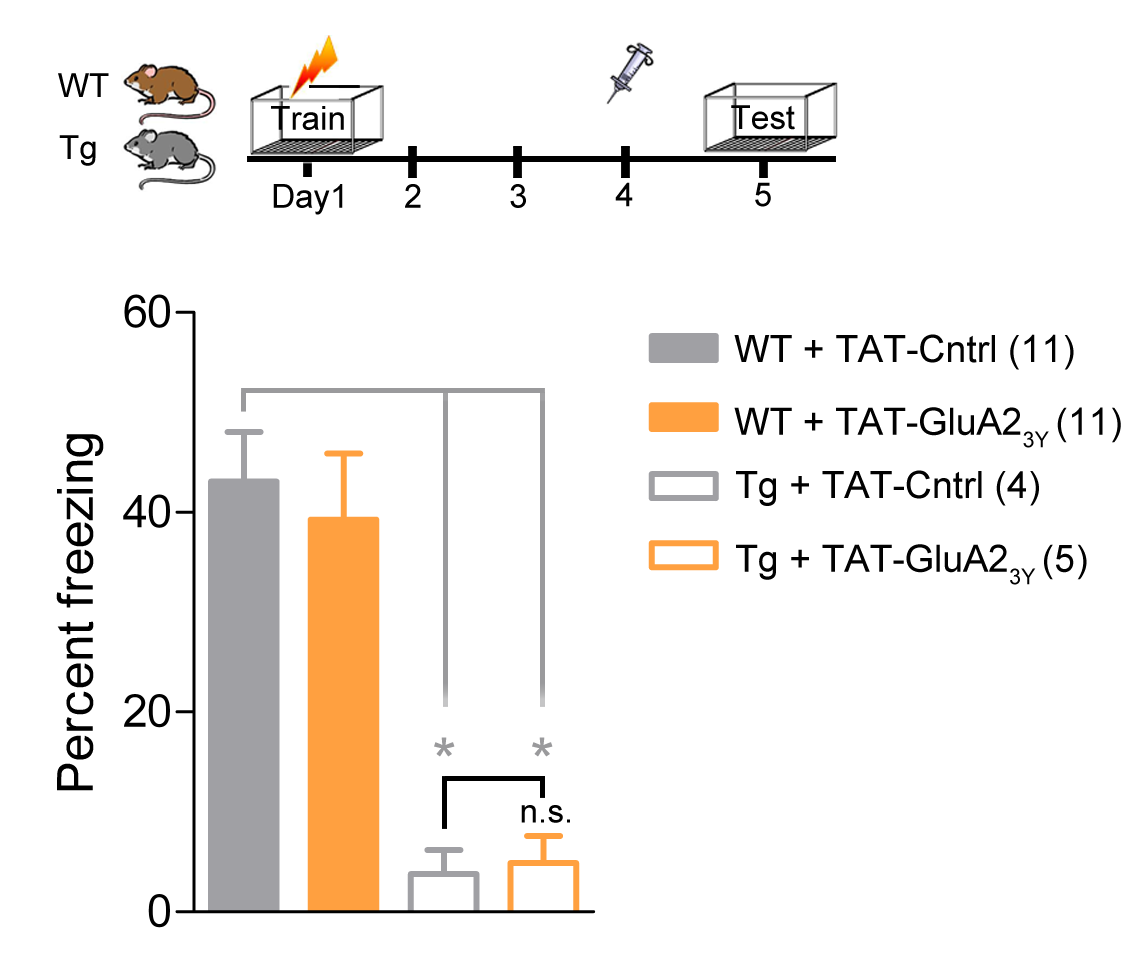
\includegraphics[width=\textwidth]{reminder2.png}
    \caption{\label{f.ad.reminder2}}
\end{figure}

\section{Discussion}
\todo{Summary of result}
\todo{Hyperactivity}
\todo{Freezing encoding: not behavioural}
\todo{Direction of causation}
\todo{\tglu rescue - how?}
